\documentclass[../document.tex]{subfiles}
\begin{document}
\chapter{Results}
\label{chap: results}
In this section, we evaluate five convolutional neural networks: the model proposed by Chavez-Garcia et al. \cite{omar2018traversability} and the four MicroResnet presented in the last chapter. We  select the best performing one based on the classification score on the test set. We show the results of the same architecture trained on regression instead of classification and prove the latter yields better results. Finally, we qualitatively evaluate the best model by predicting traversability in real-world terrains. 

% \subsection{Dataset}
% To perform classification, we selected a threshold of twenty centimeters, according to the process explained in section \ref{sec: label-patches}, on a time window  of two seconds to label the patches, meaning that a patch with an adveancement less than $20$ centimeters are labeled as \emph{no traversable} and vice-versa. For the regression thanks, we did not label the patch and directly regress on the raw advancement.

% We also assessed the model's performance on the \emph{arck rocks} map, a $10\times10$m terrain with a big rocky bump in the middle.
% The test set is composed entirely by the quarry map \ref{fig : real-maps-quarry}, a real-world terrain. Table \ref{table: maps} describes in detail the configuration used in to generate all datasets.


\section{Quantitative results}
\subsection{Model selection}
We compare the four different MicroRenset architectures \ref{subsec :micro-resnets} and the Original CNN \ref{subsec : vanilla-cnn} propose in the original work \cite{omar2018traversability} on classification. The dataset is labeled as described in \ref{sec : label-patches}. We run five experiments per architecture, and we select the best performing network using as a metric the ROC AUC. Table \ref{tab : models-results-comparison} shows the results for each architecture. The best performing model is MicroResNet7x7-SE with a ROC AUC of 0.896 on the test set. We suggest that the big kernel size allows the network to extrapolate more gound features in the first layer. Also, the results demonstrate the performance boots given by the Squeeze and Excitation. MicroResNet7x7-SE  gains a huge boost of $0.021$ compared to MicroResNet7x7.
\begin{table*}[ht]
  \centering
  \ra{1.2}
  \begin{tabular}{@{}lcccc@{}}
    \toprule
    Model & \multicolumn{2}{c}{ROC AUC} & Params \\ 
    \cline{1-4}
    & Mean & Top &  \\ 
    \cline{1-4}
    Original (baseline)  & 0.892& 0.890 &  974,351 \\
    MicroResnet3x3 & 0.881 & 0.883 & 302,610 \\
    MicroResnet3x3-SE & 0.883 & 0.888 & 313,64\\
    MicroResnet7x7 & 0.867 & 0.875 &  303,250\\
    MicroResnet7x7-SE &0.888 & \textbf{0.896} & 314,28\\
    \bottomrule   
  \end{tabular}
  \caption{Comparison of the four MicroResnet architectures \ref{fig : microresnet} and the original convolutional neural network (Original CNN) proposed in the original work \cite{omar2018traversability} on the test set. We run five experiments per architecture, we show the average and the top score for each metric. The best model is MicroResNet7x7-SE.}
  \label{tab : models-results-comparison}
\end{table*}
\section{Classification results}
Table \ref{tab : classification-results} table shows in deep the  MicroResNet7x7-SE's performance on different datasets. We obstain an $95\%$ accuracy and $0.96$ AUC on the validation set and $88\%$ accuracy and $0.89$ AUC on the test set.
\begin{table*}[htbp]
    \centering
    \ra{1.2}
    \begin{tabular}{@{}llccccc@{}}
    \toprule
    % \multicolumn{8}{c}{Quantitative evaluation in simulation} \\
    \multicolumn{2}{c}{Dataset} && \multicolumn{2}{c}{MicroResNet7x7-SE} & Size(m) & Resolution(cm/px) \\
    \cmidrule{1-2} \cmidrule{4-5}
    Type     &  Name  & Samples & ACC  &  AUC    & & \\
    \toprule
      \multirow{3}{*}{Synthetic}  & Training   & 429312 & - & - & $10\times10$ & 2\\
      &  Validation   & 44032 &  95.2 \% &  0.961 & $10\times10$ & 2 \\
      & Arc Rocks & 37273 &  85.5 \% &  0.888 & $10\times10$ & 2 \\
      \cmidrule{2-7}
    Real\\evaluation & Quarry & 36224 &  88.2 \%&  0.896& $32\times32$ & 2\\
    % \multirow{1}{*}{\makecell[l]{Real\\evaluation}} & Quarry & 36224 &  88.2 \%&  0.896& & 2\\
    \bottomrule   
\end{tabular}
\caption{Classification results of MicroResNet7x7-SE on different datasets.}
\label{tab : classification-results}
\end{table*}
\section{Regression Results}
Using MicroResNet7x7-SE as regressor also yield decent results. The model scores a MSE of $0.006$ on the validation and $0.020$ on the test set. Table \ref{tab : regression-results} shows in detail the score for each dataset.
\begin{table*}[htbp]
    \centering
    \ra{1.2}
    \begin{tabular}{@{}llcccc@{}}
    \toprule
    % \multicolumn{8}{c}{Quantitative evaluation in simulation} \\
    \multicolumn{2}{c}{Dataset} & & \multicolumn{1}{c}{MicroResNet7x7-SE} & Size & Resolution(cm/px) \\
    \cmidrule{1-2} \cmidrule{4-5}
    Type     &  Name  & Samples & MSE      & \\
    \toprule
      \multirow{3}{*}{Synthetic}  & Training  &  - & - &$10\times10$  & 2\\
      &  Validation   & 44032 &  0.006  &  $10\times10$ & 2 \\
      & Arc Rocks & 37273 & 0.020  &  $10\times10$& 2 \\
      \cmidrule{2-6}
    Real\\evaluation & Quarry & 36224 &  0.022 & $32\times32$ & 2\\
    % \multirow{1}{*}{\makecell[l]{Real\\evaluation}} & Quarry & 36224 &  88.2 \%&  0.896& & 2\\
    \bottomrule   
\end{tabular}
\caption{Regression results of MicroResNet7x7-SE on different datasets.}
\label{tab : regression-results}
\end{table*}
Figure \ref{fig : regression-preds-targs} plots the real advancement against the regressor output for the test set. In most cases the model did not correctly predict the advancement.
\begin{figure}[htbp]
  \centering
  \begin{subfigure}[b]{1\linewidth}
    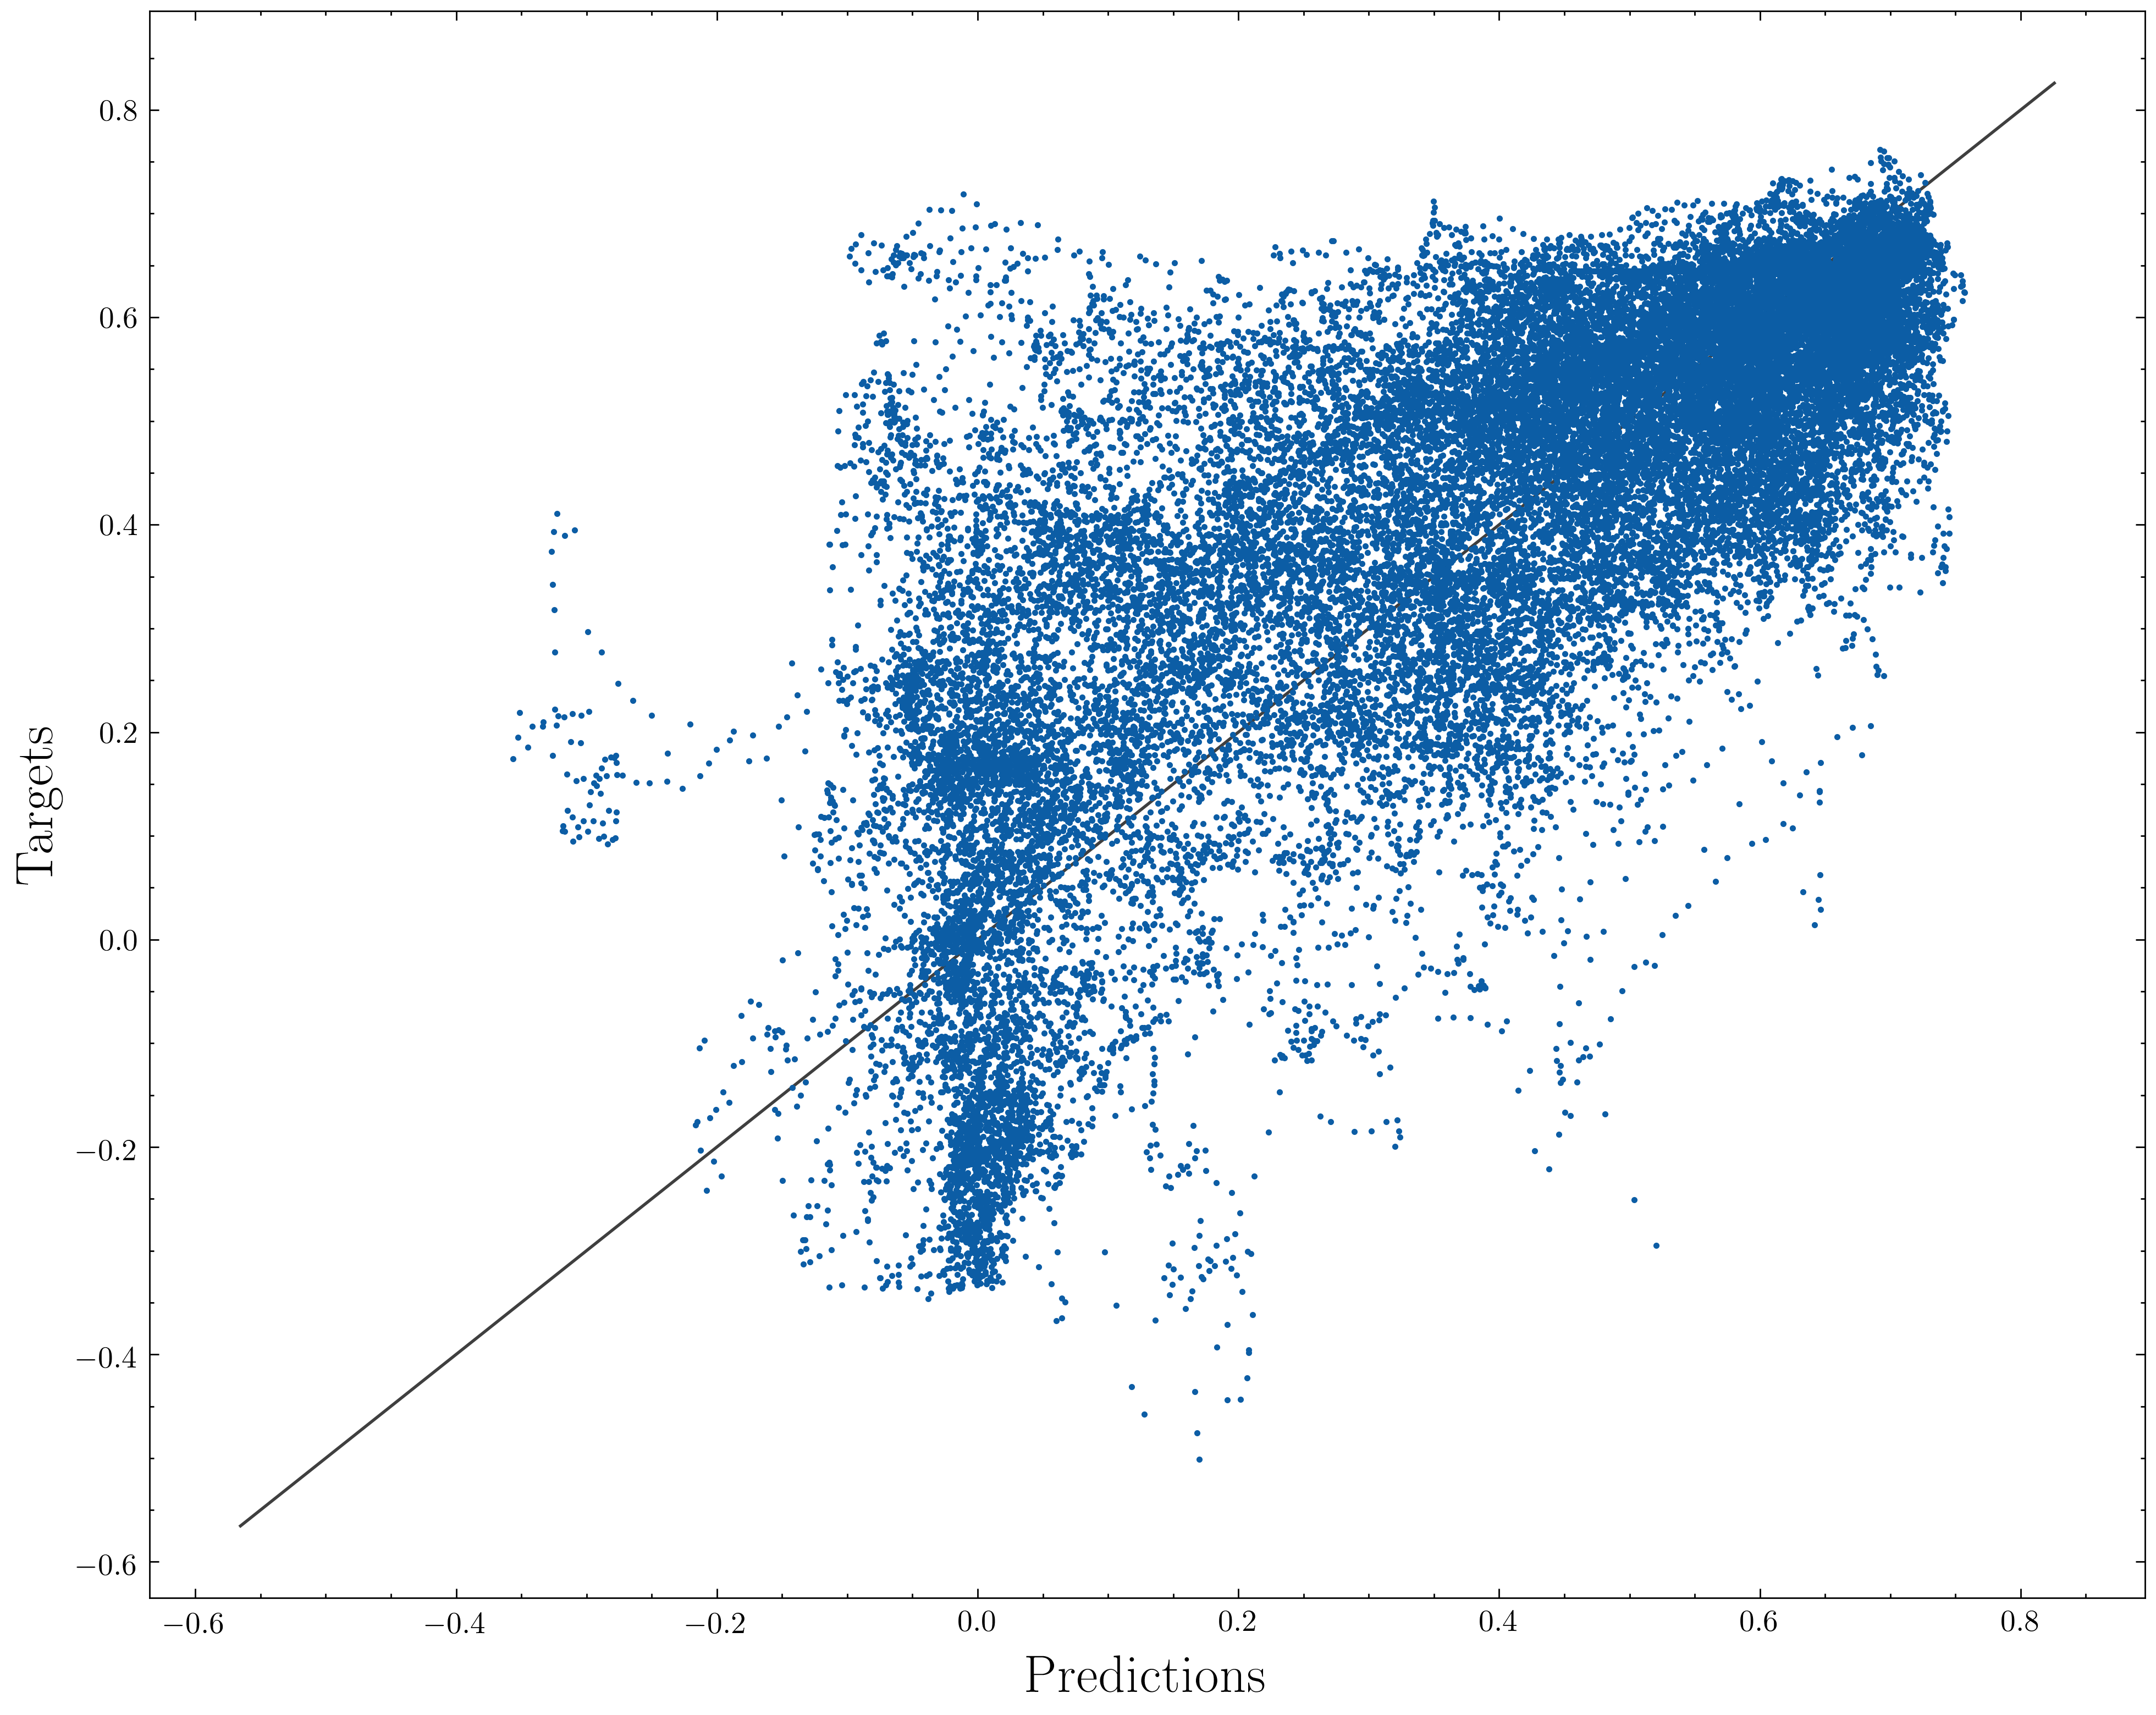
\includegraphics[width=\linewidth]{../img/4/regression_scatter.png} 
  \end{subfigure}
  \caption{RReal advancement against the regressor output for the test set. Most of the points are far away to the diagonal line showing that the regressor predicts the wrong advancement in many cases.}
  \label{fig : regression-preds-targs}
\end{figure}
The regressor has several advantages compared to the classifier, First, since we can use the same model to classify patches with a different threshold. This is done by seeing if the predicted advancement is greater or lower than a threshold. Regression is a usually feasible solution. For example, if we need to consider multiple thresholds. Classification requires the training of one classifier per threshold while regression can evaluate always the same model.

However, if we fixed a threshold, the same exactly architecture trained directly to predict traversability outperforms the regressor. Table \ref{tab : reg-clas} shows the accuracy of two MicroResNet7x7-SE on classification and regression after a threshold of twenty centimeters is selected. The classifier outperformed the regressor. For this reason, we decided to evaluate the MicroResNet7x7-SE classifier. 
\begin{table*}[htbp]
  \centering
  \ra{1.2}
  \begin{tabular}{@{}lcc@{}}
  \toprule
  &  Regression & Classification  \\
 & \multicolumn{2}{c}{ACC} \\ 
  \cline{2-3}
   Top & $72.8\%$ & \textbf{88.2\%} \\
   Mean & $73.6\%$ & \textbf{87.8\%} \\
  \bottomrule   
\end{tabular}
\caption{Regression and classification accuracy for the same model,  MicroResNet7x7-SE, on a threshold of $20$cm. The regression accuracy is computed using its output labeled with the selected threshold and the binary targets from the classification dataset. This mimic the situaion when the fixed a miniuim advancement for the robot.In this case, the classifier outperforms the regressor.}
\label{tab : reg-clas}
\end{table*}
% Moreover, we would like to also show the different steps we made to reach this result. The following table shows the metric's score without any data-augmentation.
% Adding dropout increases the results.
% With dropout plus coarse dropout.
We evaluate the classifier predictions by plotting the traversability probability on different maps in 3D. We used a sliding window to extract the patches to generate the patches. Then, we created a texture based on the traversable probability. For each map, we evaluated four headings.
%  robot movingfrom bottom to top, top to bottom, left to right and right to left since those are the most human understandable. By using those angles, we can optimize the cropping process since to avoid rotate each patch based on the Krock's head position. Instead, we can just rotate the entire map beforehand. 
subsection{Quarry}
We first evaluate the test set composed by the quarry map  $32\times32$m  and with a maximum height of $10$m. We expect the trail on the slopes to be traversable at almost any headings, especially when Krock move from left to right and vice-versa. The top part should be hard to traverse in almost any case. Figure \ref{fig : quarry-trav} shows the traversability probability directly on the map. 
\todo[inline]{some where place the colormap bar}
\begin{figure} [htbp]
\centering
\begin{subfigure}[b]{0.45\textwidth}
  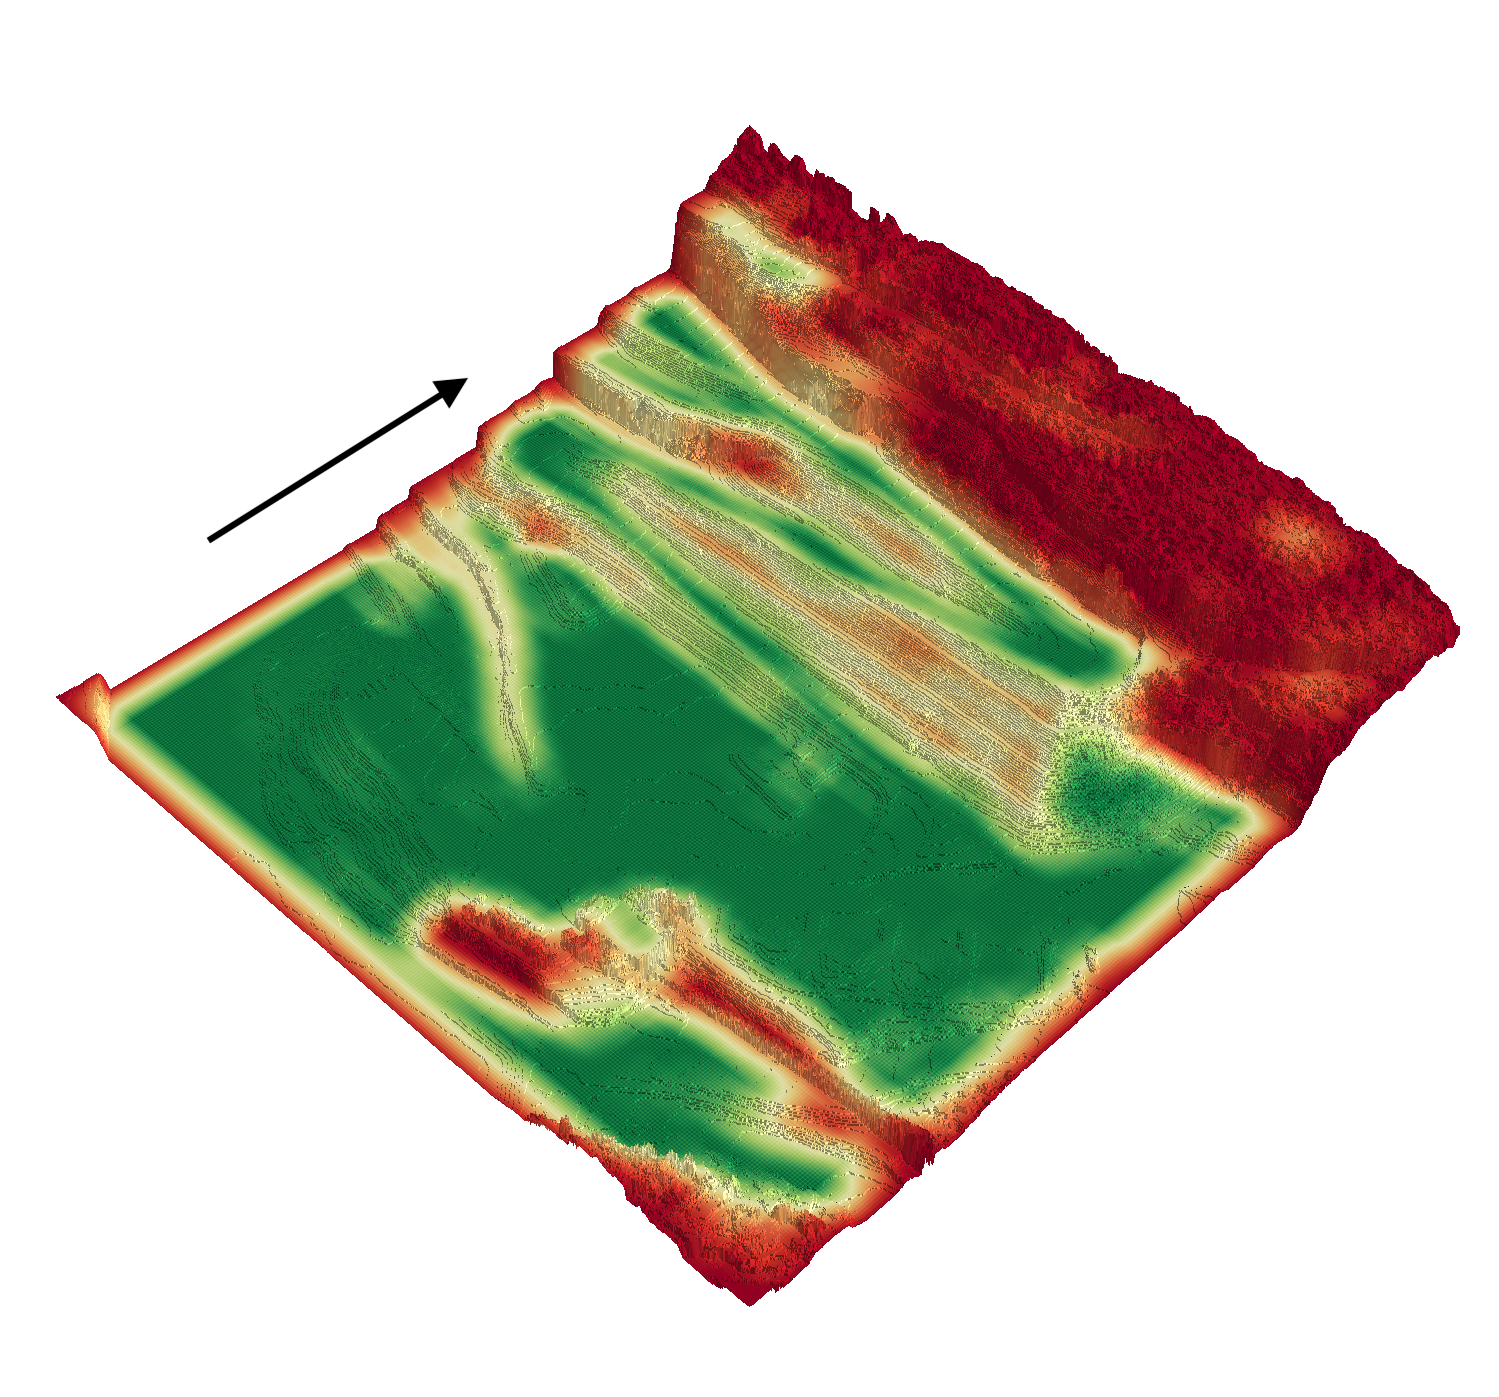
\includegraphics[width=\linewidth]{../img/4/traversability/quarry/-270.png} 
  \subcaption{Robot moving from bottom to top} 
  % \label{fig: quarry-b2t}
\end{subfigure}
\begin{subfigure}[b]{0.45\textwidth}
    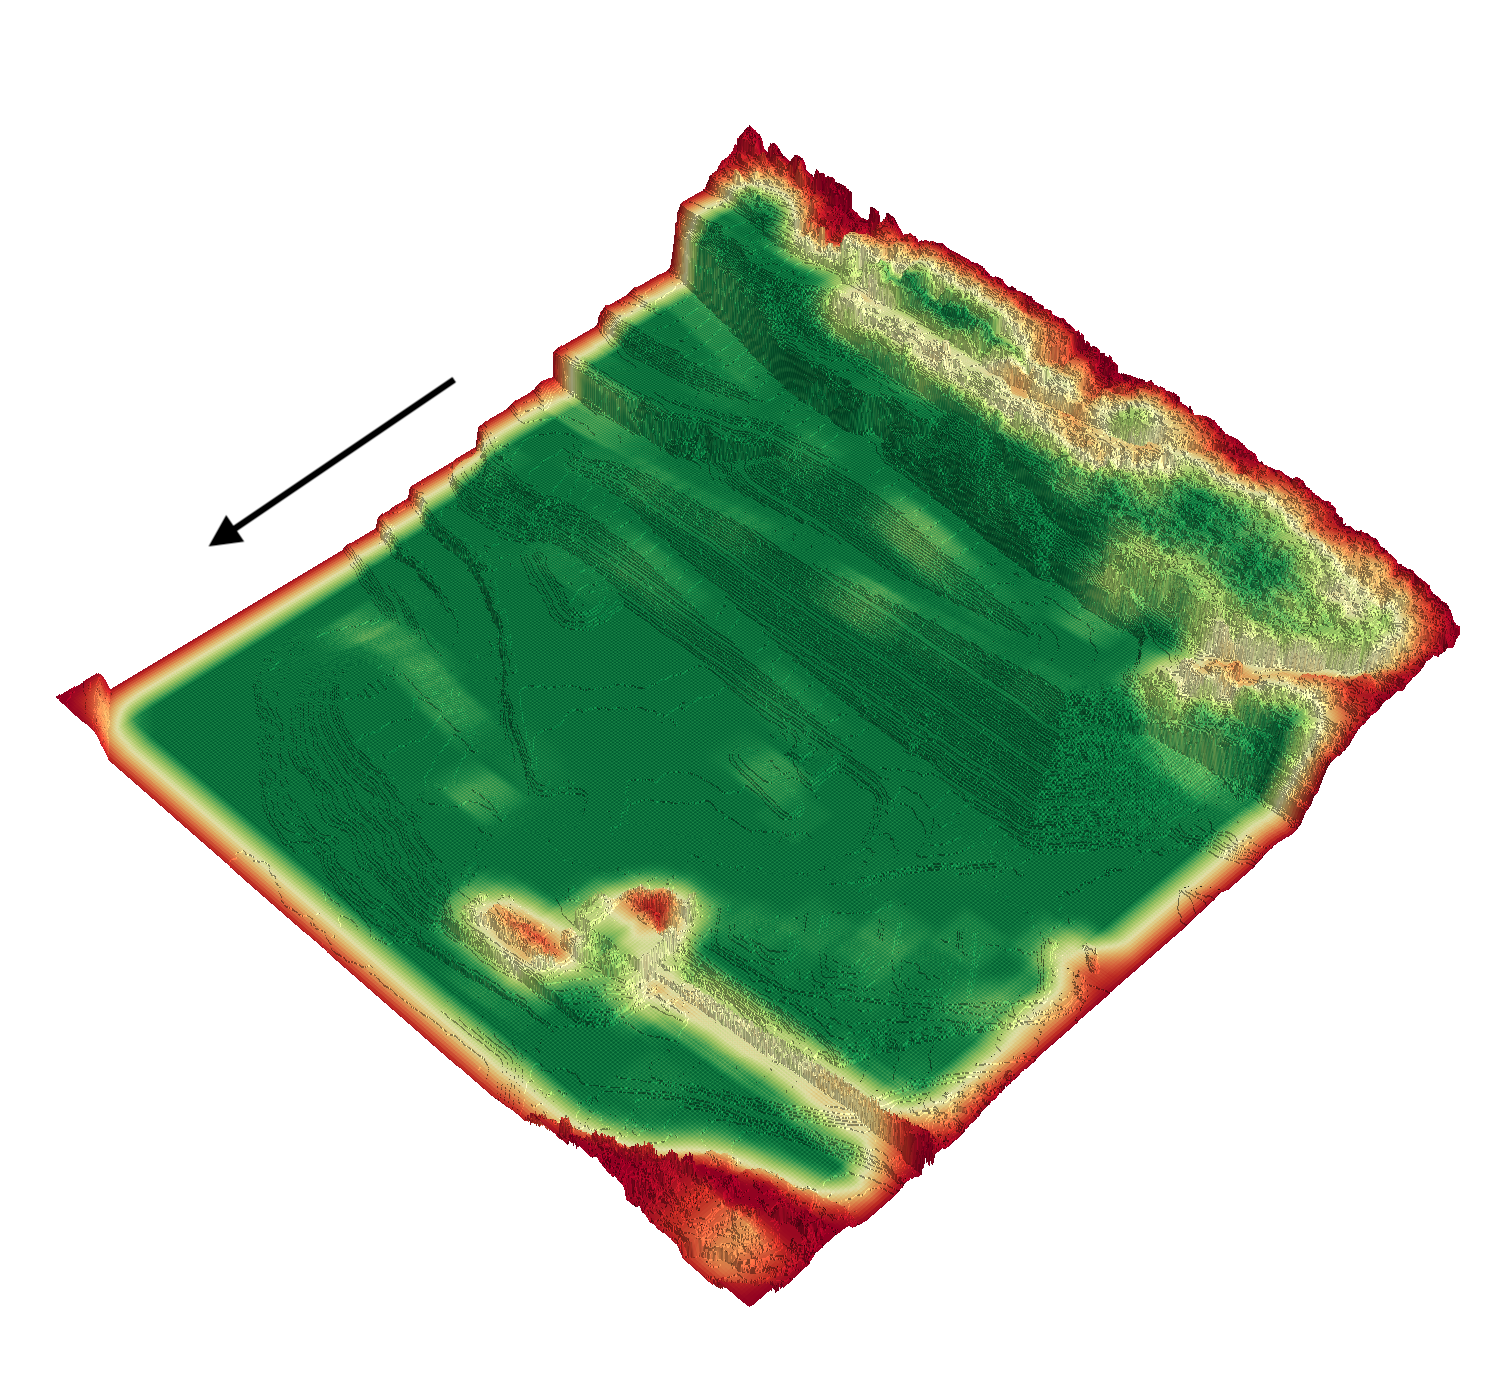
\includegraphics[width=\linewidth]{../img/4/traversability/quarry/-90.png}
    \subcaption{Robot moving from top to bottom} 
    % \label{fig: quarry-t2b}
\end{subfigure}
\begin{subfigure}[b]{0.45\textwidth}
  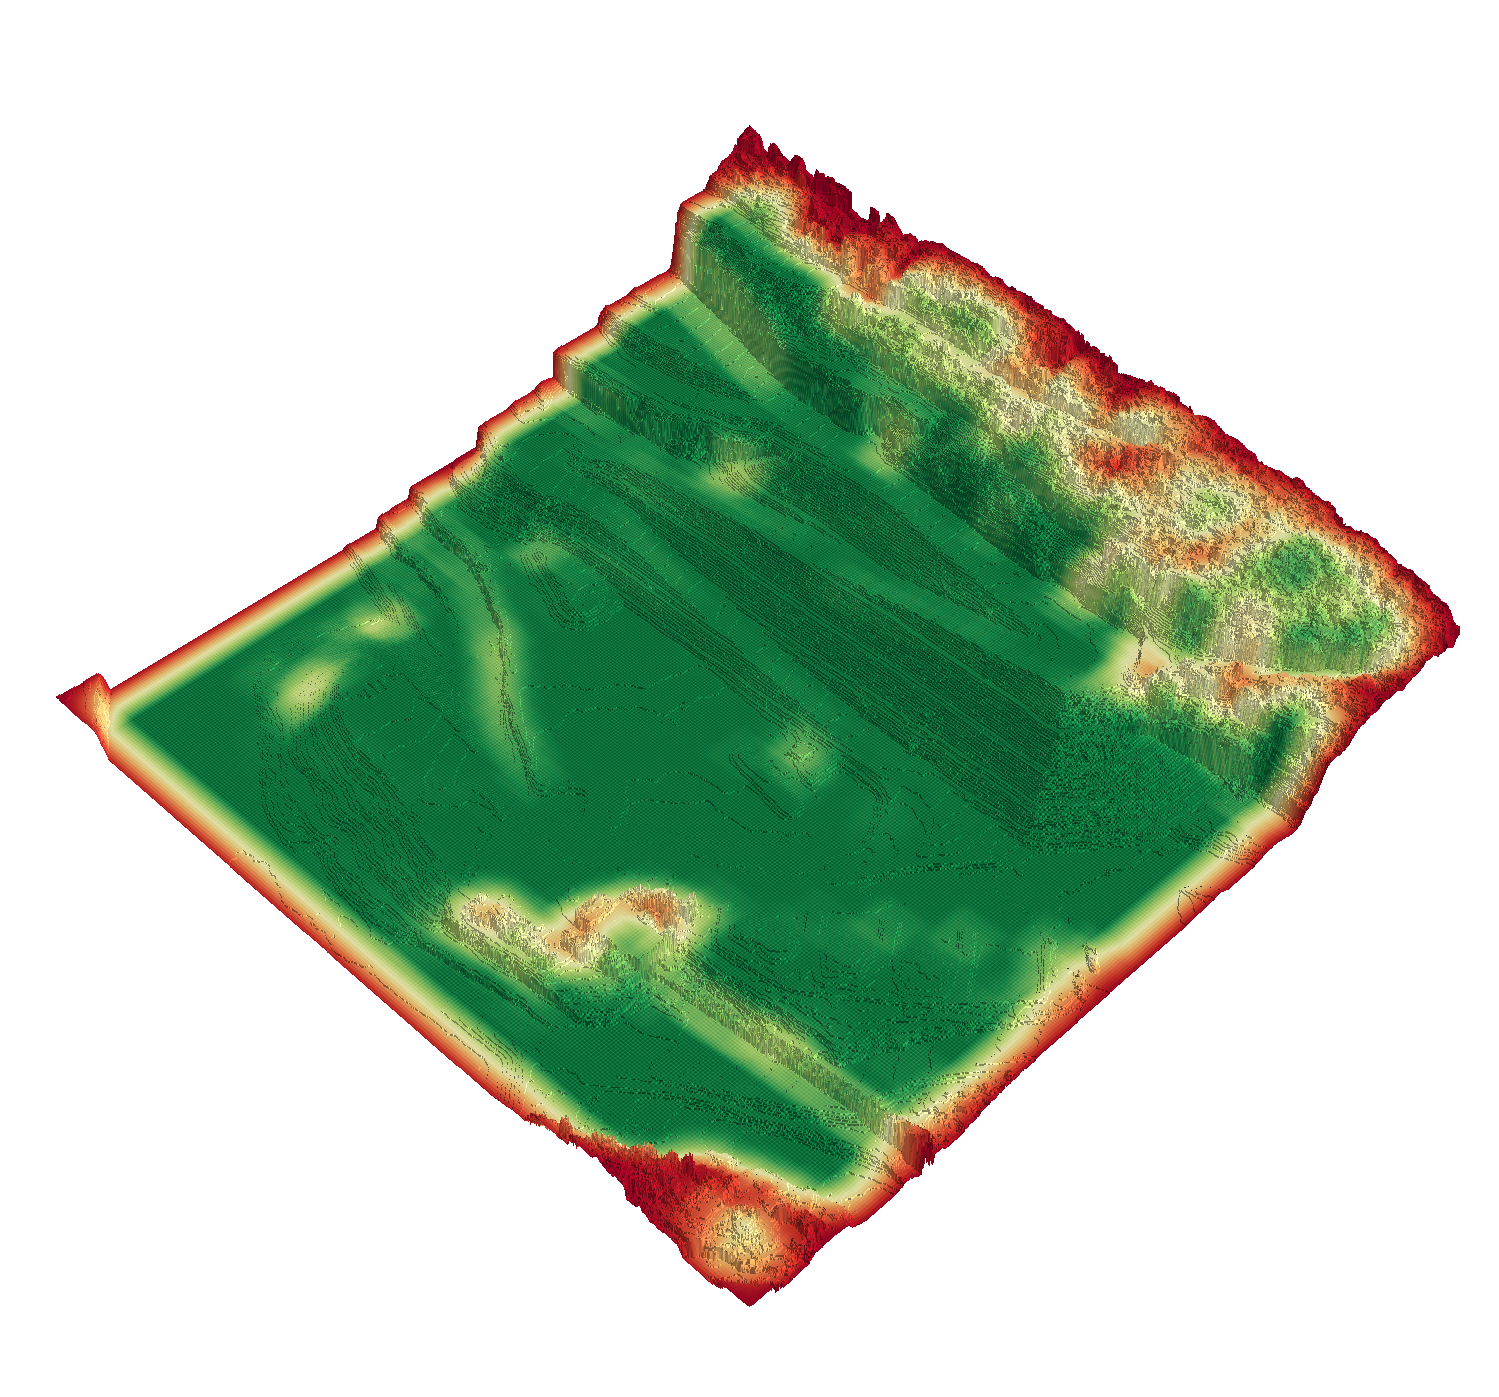
\includegraphics[width=\linewidth]{../img/4/traversability/quarry/-0.png}
  \subcaption{Robot moving from left to right}   
  % \label{fig: quarry-l2r}
\end{subfigure}
\begin{subfigure}[b]{0.45\textwidth}
    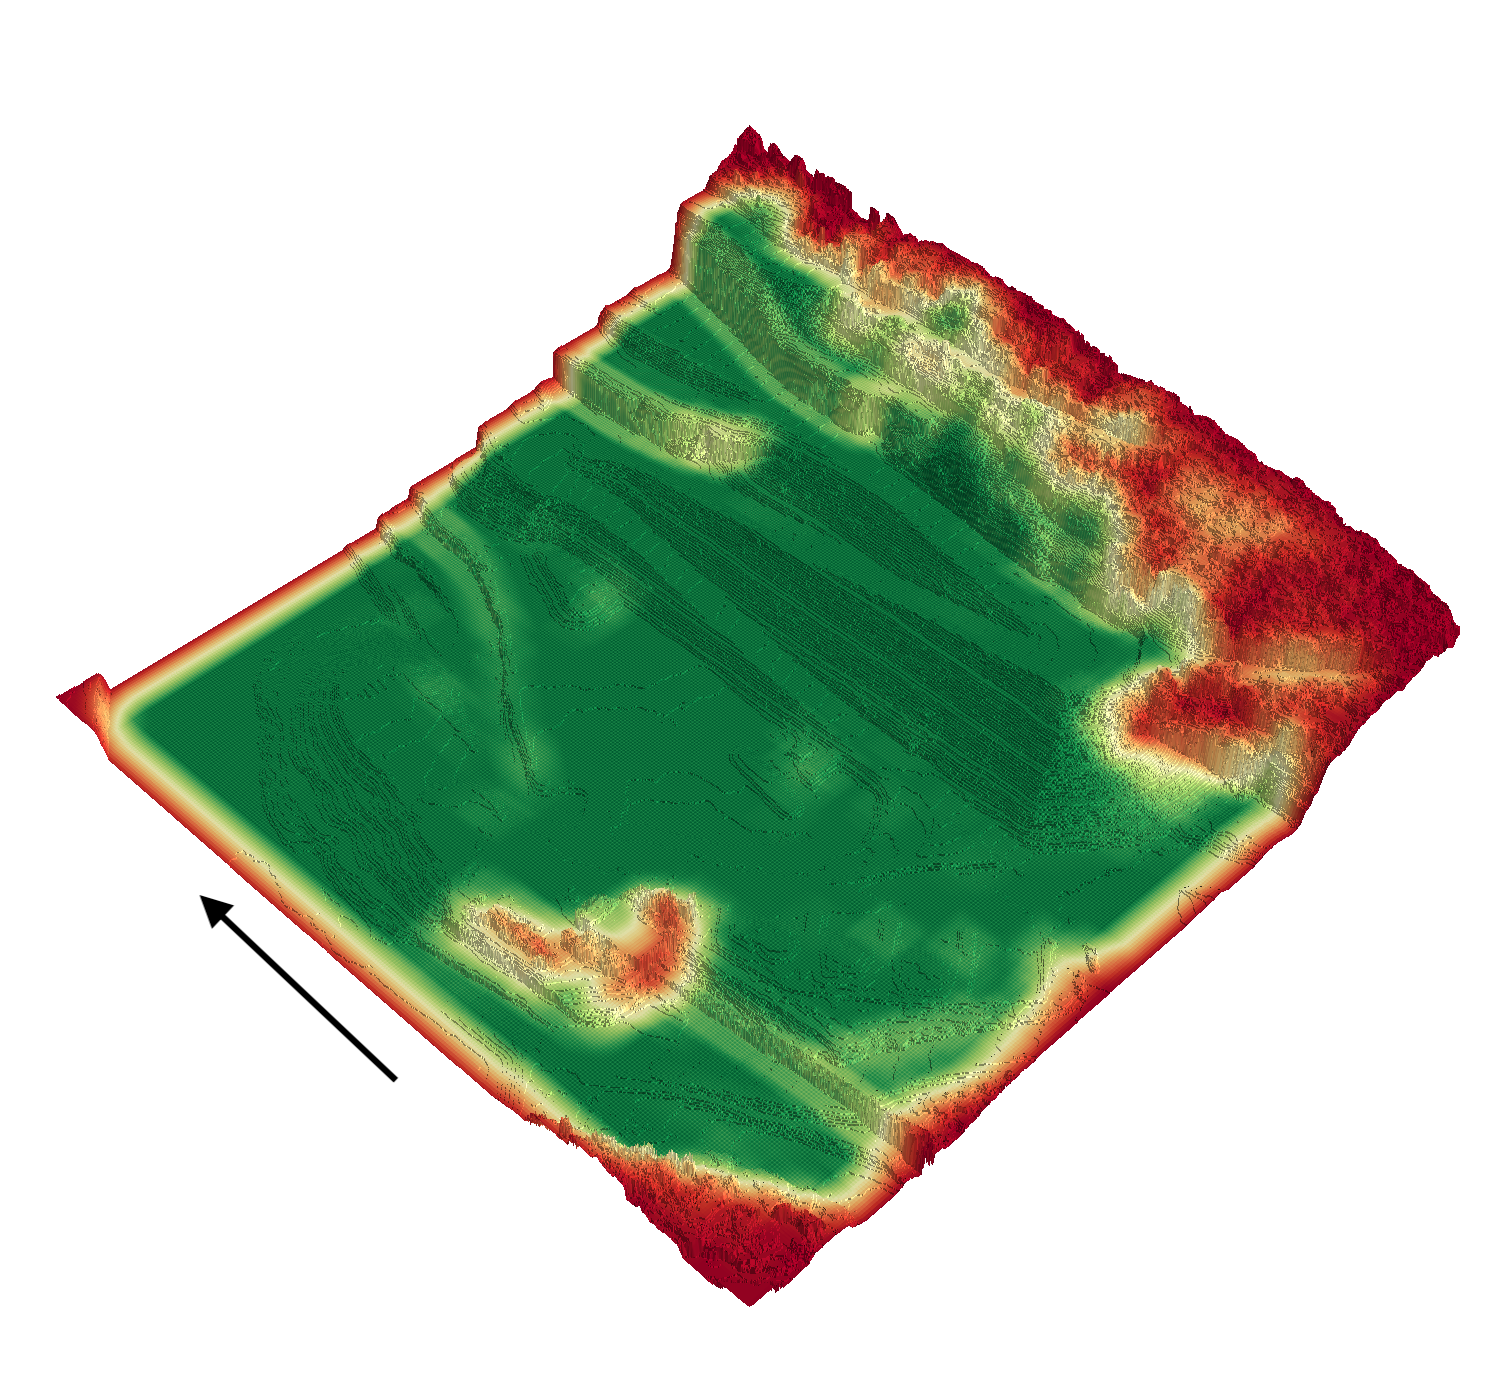
\includegraphics[width=\linewidth]{../img/4/traversability/quarry/-180.png}  
    \subcaption{Robot moving from right to left} 
    % \label{fig: quarry-r2l}
\end{subfigure}
\caption{Traversability probability on the test set, a quarry $32\times 32$m and a maximum height of $10$m, for different Krock's orientations. }
\label{fig : quarry-trav}
\end{figure}
 Correctly, the lower part of the map, composed by flat regions, is labeled with high confidence as traversable in all rotations. On the other hand, the traversability of the slopes and the bumps on the top region depends on the robot orientation.

\subsection{Bars}
Bars is a map composed of walls with different heights, thus we expected to be mostly not traversable at different headings. Figure \ref{fig : bars-trav} shows the traversability probabilities on the terrain.

\begin{figure} [htbp]
  \centering
  \begin{subfigure}[b]{0.45\textwidth}
    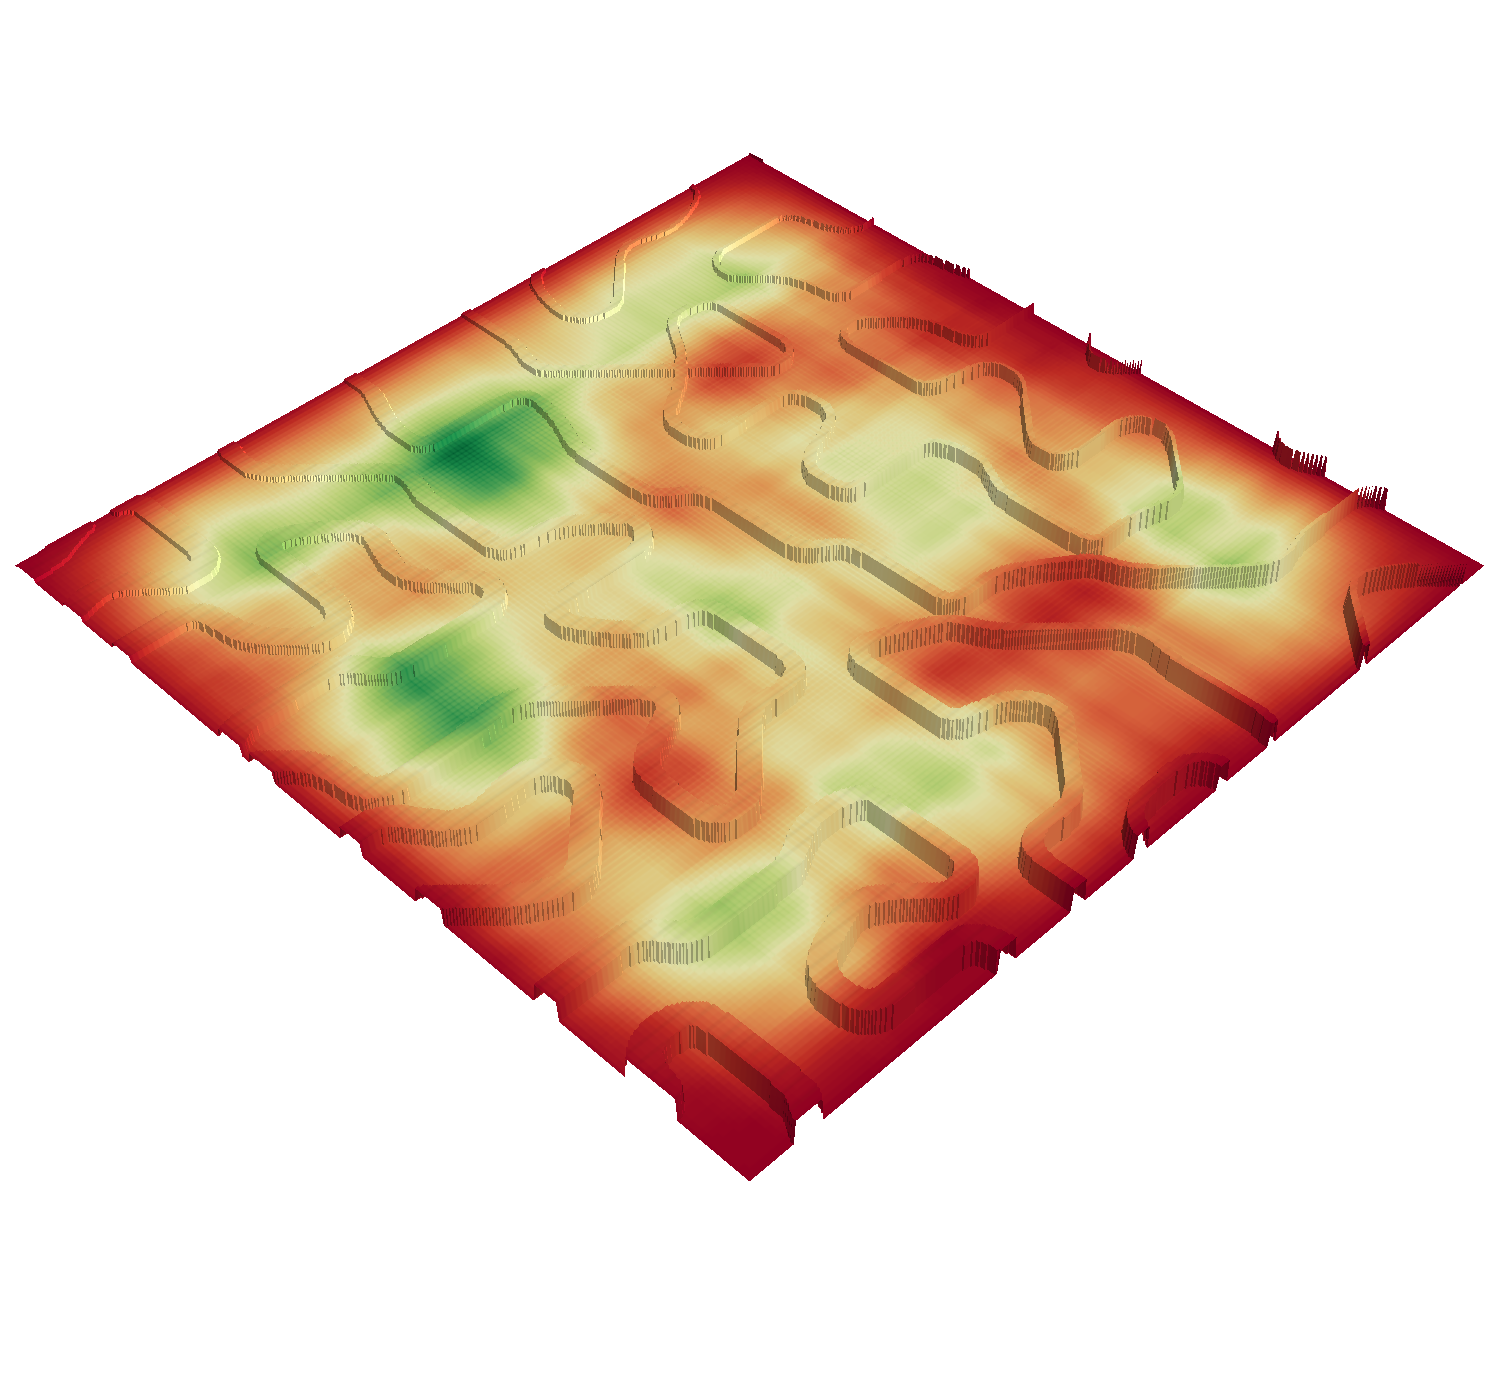
\includegraphics[width=\linewidth]{../img/4/traversability/bars/-270.png} 
    \subcaption{Robot moving from bottom to top} 
    % \label{fig: bars-b2t}
  \end{subfigure}
  \begin{subfigure}[b]{0.45\textwidth}
      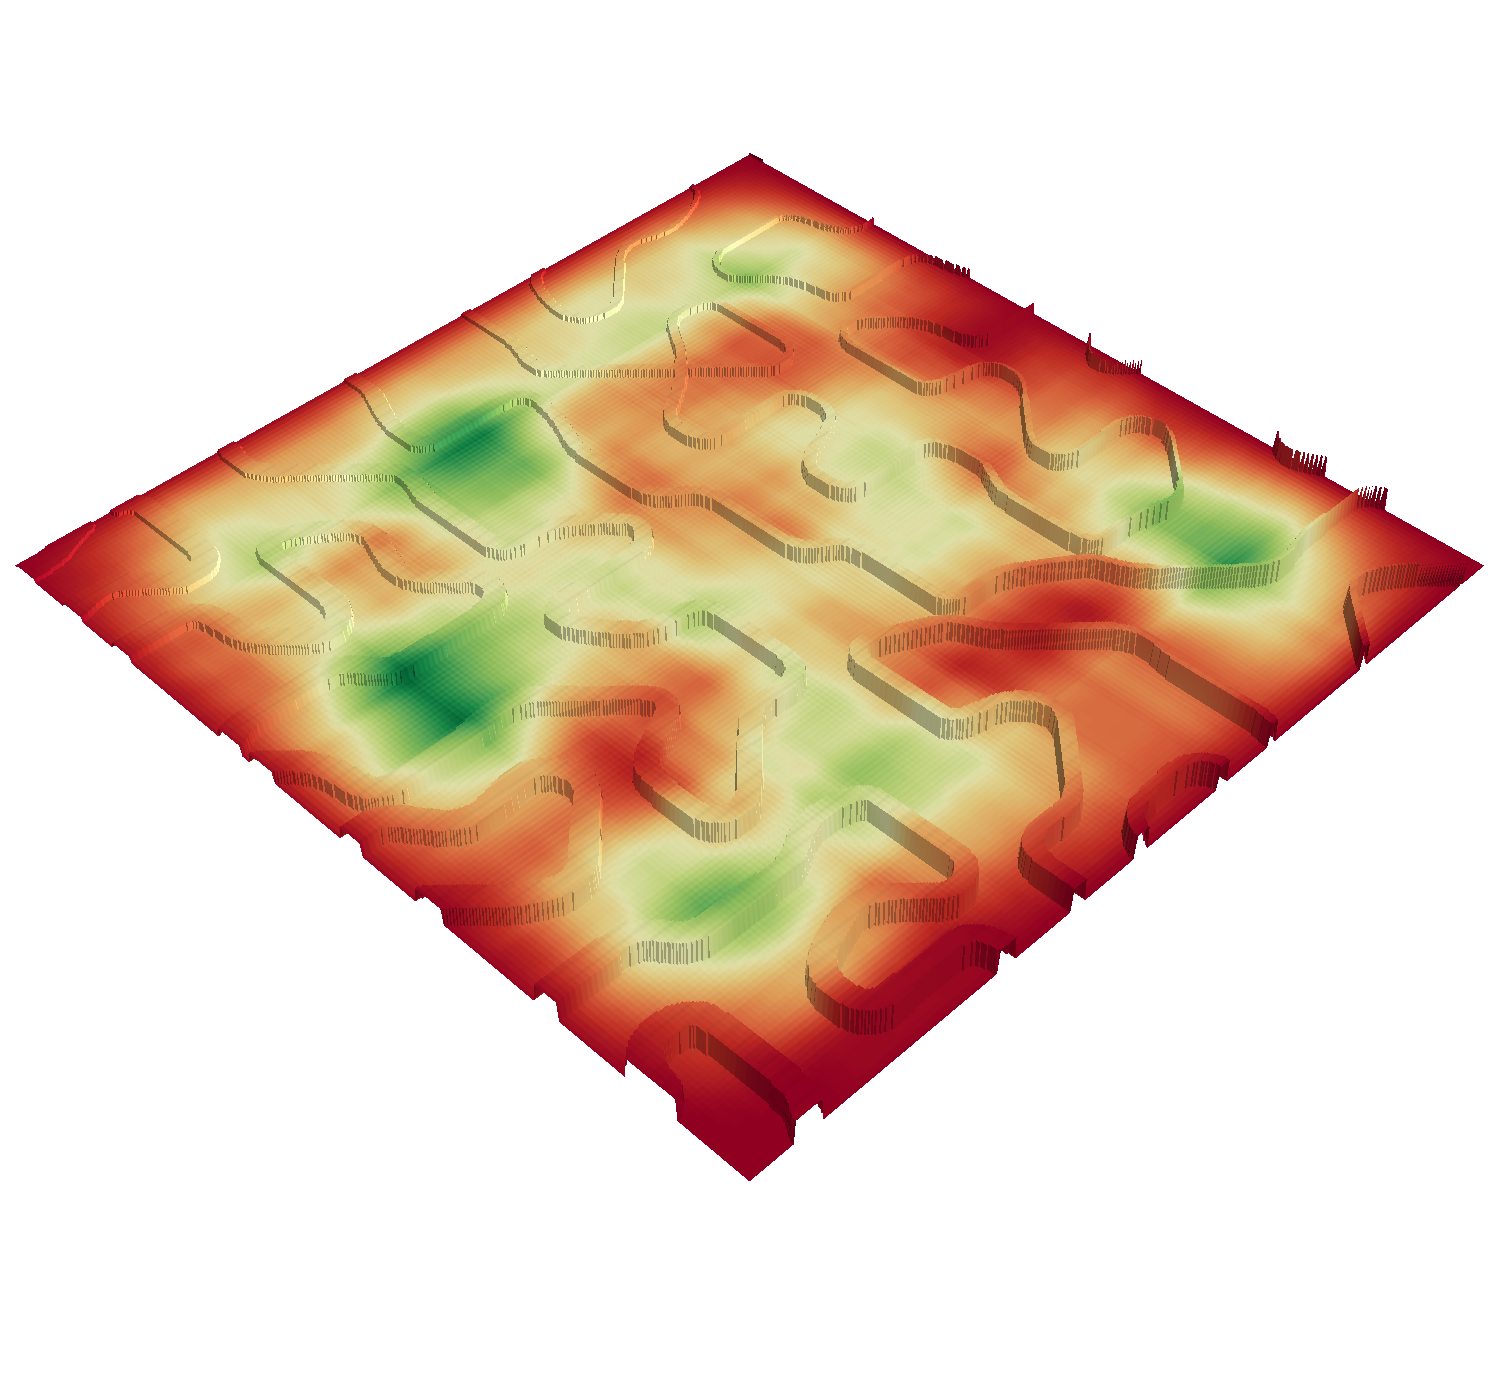
\includegraphics[width=\linewidth]{../img/4/traversability/bars/-90.png}
      \subcaption{Robot moving from top to bottom} 
      % \label{fig: bars-t2b}
  \end{subfigure}
  \begin{subfigure}[b]{0.45\textwidth}
    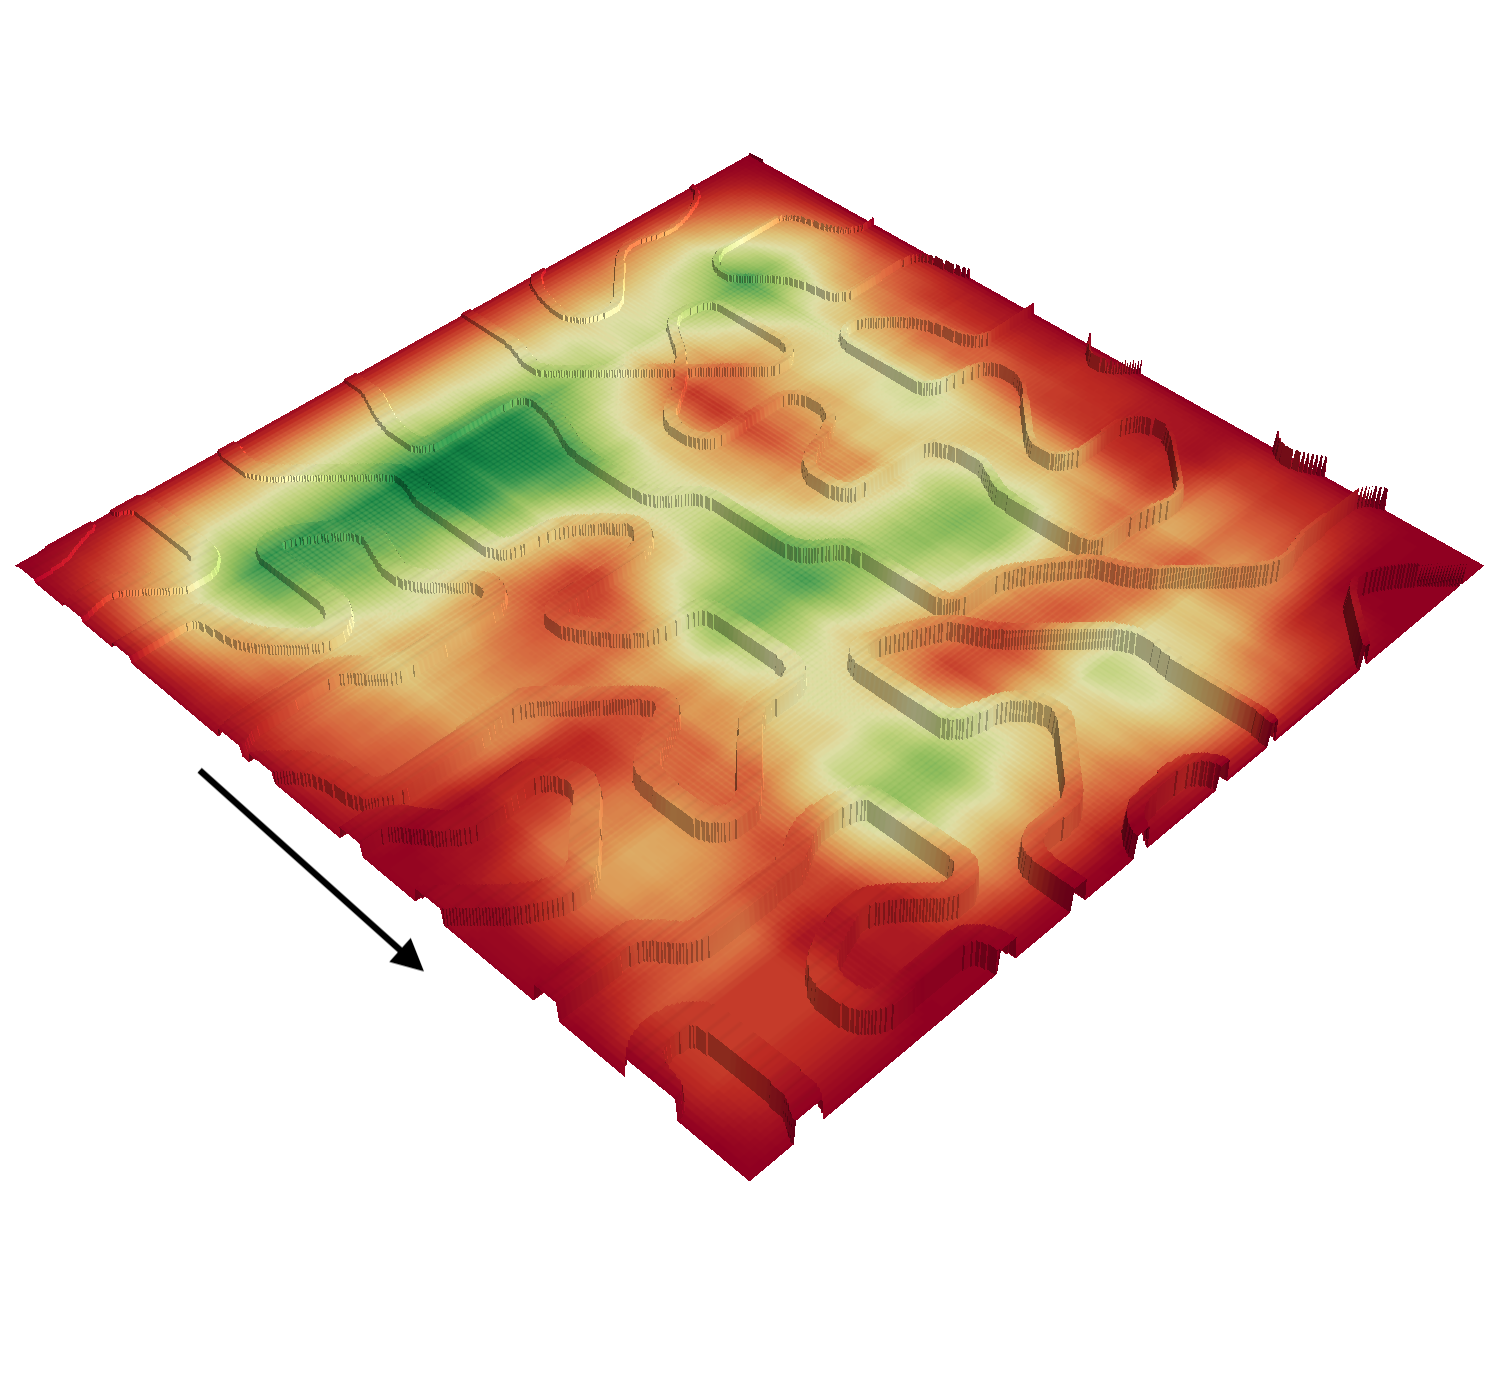
\includegraphics[width=\linewidth]{../img/4/traversability/bars/-0.png}
    \subcaption{Robot moving from left to right}   
    % \label{fig: bars-l2r}
  \end{subfigure}
  \begin{subfigure}[b]{0.45\textwidth}
      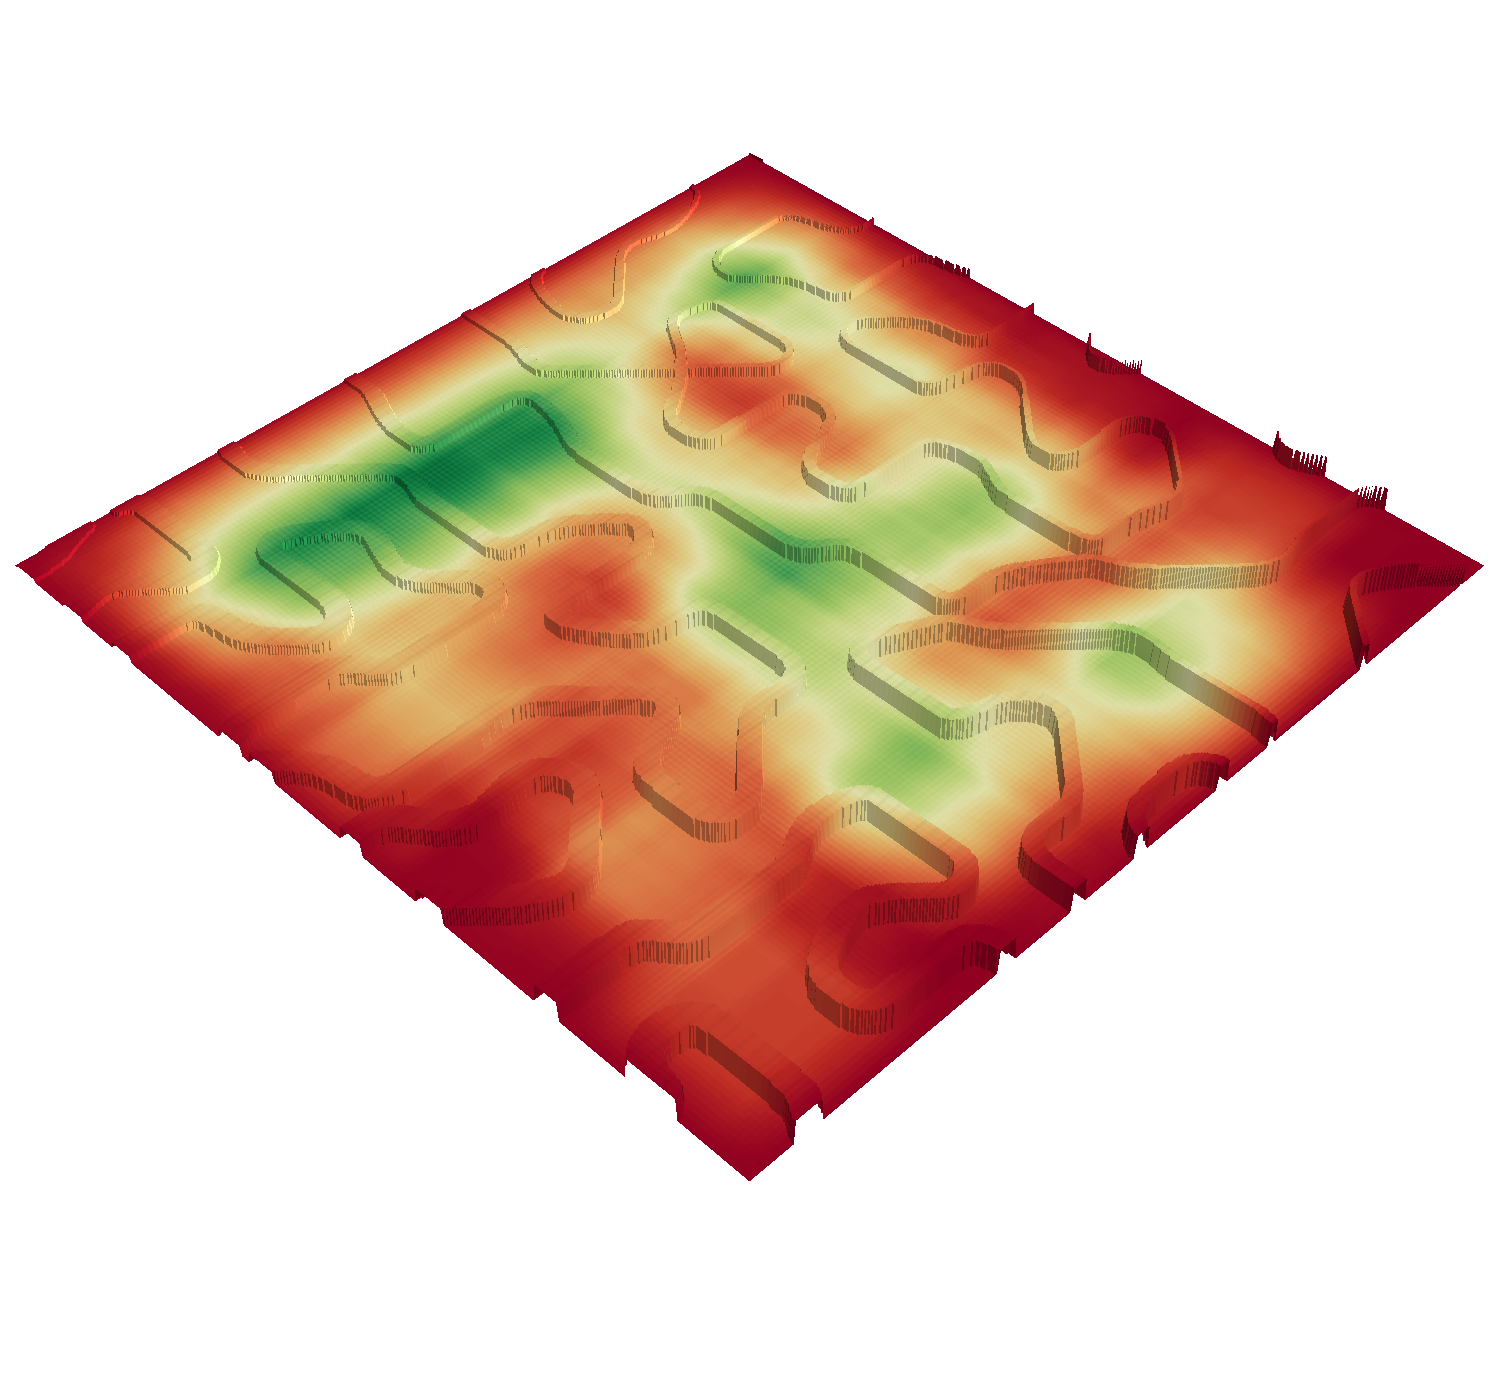
\includegraphics[width=\linewidth]{../img/4/traversability/bars/-180.png}  
      \subcaption{Robot moving from right to left} 
      % \label{fig: bars-r2l}
  \end{subfigure}
  \caption{Traversability probability on the bars map, a $10\times 10$m , for different Krock's orientations.}
  \label{fig : bars-trav}
  \end{figure}
Due to the high number of not traversable walls, this is a hard map to traverse the robot . Interesting, we can identify a corridor near the bottom center of the maps. This region shows how the model correctly label those patches depending on the orientation. Figure \ref{fig : bars-tunnel-trav} highlights this detail.

\begin{figure} [htbp]
  \centering
  \begin{subfigure}[b]{0.23\textwidth}
    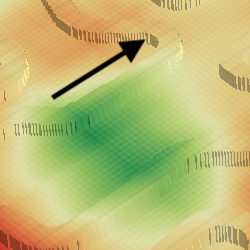
\includegraphics[width=\linewidth]{../img/4/traversability/bars/tunnel/-270-crop.png} 
    % \subcaption{Robot moving from bottom to top} 
    % \label{fig: bars-b2t}
  \end{subfigure}
  \begin{subfigure}[b]{0.23\textwidth}
      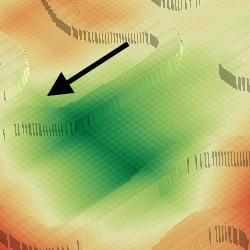
\includegraphics[width=\linewidth]{../img/4/traversability/bars/tunnel/-90-crop.png}
      % \subcaption{Robot moving from top to bottom} 
      % \label{fig: bars-t2b}
  \end{subfigure}
  \begin{subfigure}[b]{0.23\textwidth}
    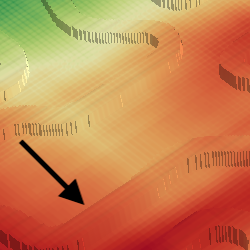
\includegraphics[width=\linewidth]{../img/4/traversability/bars/tunnel/-0-crop.png}
    % \subcaption{Robot moving from left to right}   
    % \label{fig: bars-l2r}
  \end{subfigure}
  \begin{subfigure}[b]{0.23\textwidth}
      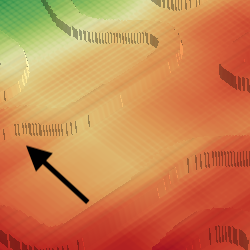
\includegraphics[width=\linewidth]{../img/4/traversability/bars/tunnel/-180-crop.png}  
      % \subcaption{Robot moving from right to left} 
      % \label{fig: bars-r2l}
  \end{subfigure}
  \caption{Detail of a region in the bars map where there are two walls forming a corridor. When the robot is  following the trail the region is label as traversable.}
  \label{fig : bars-tunnel-trav}
  \end{figure}

\subsection{Small village}
We apply the same procedure to evaluate the network on a $10\times10$m small village map. Figure \ref{fig : small-village-trav} describes its traversability for four different rotations.

\begin{figure} [htbp]
  \centering
  \begin{subfigure}[b]{0.45\textwidth}
    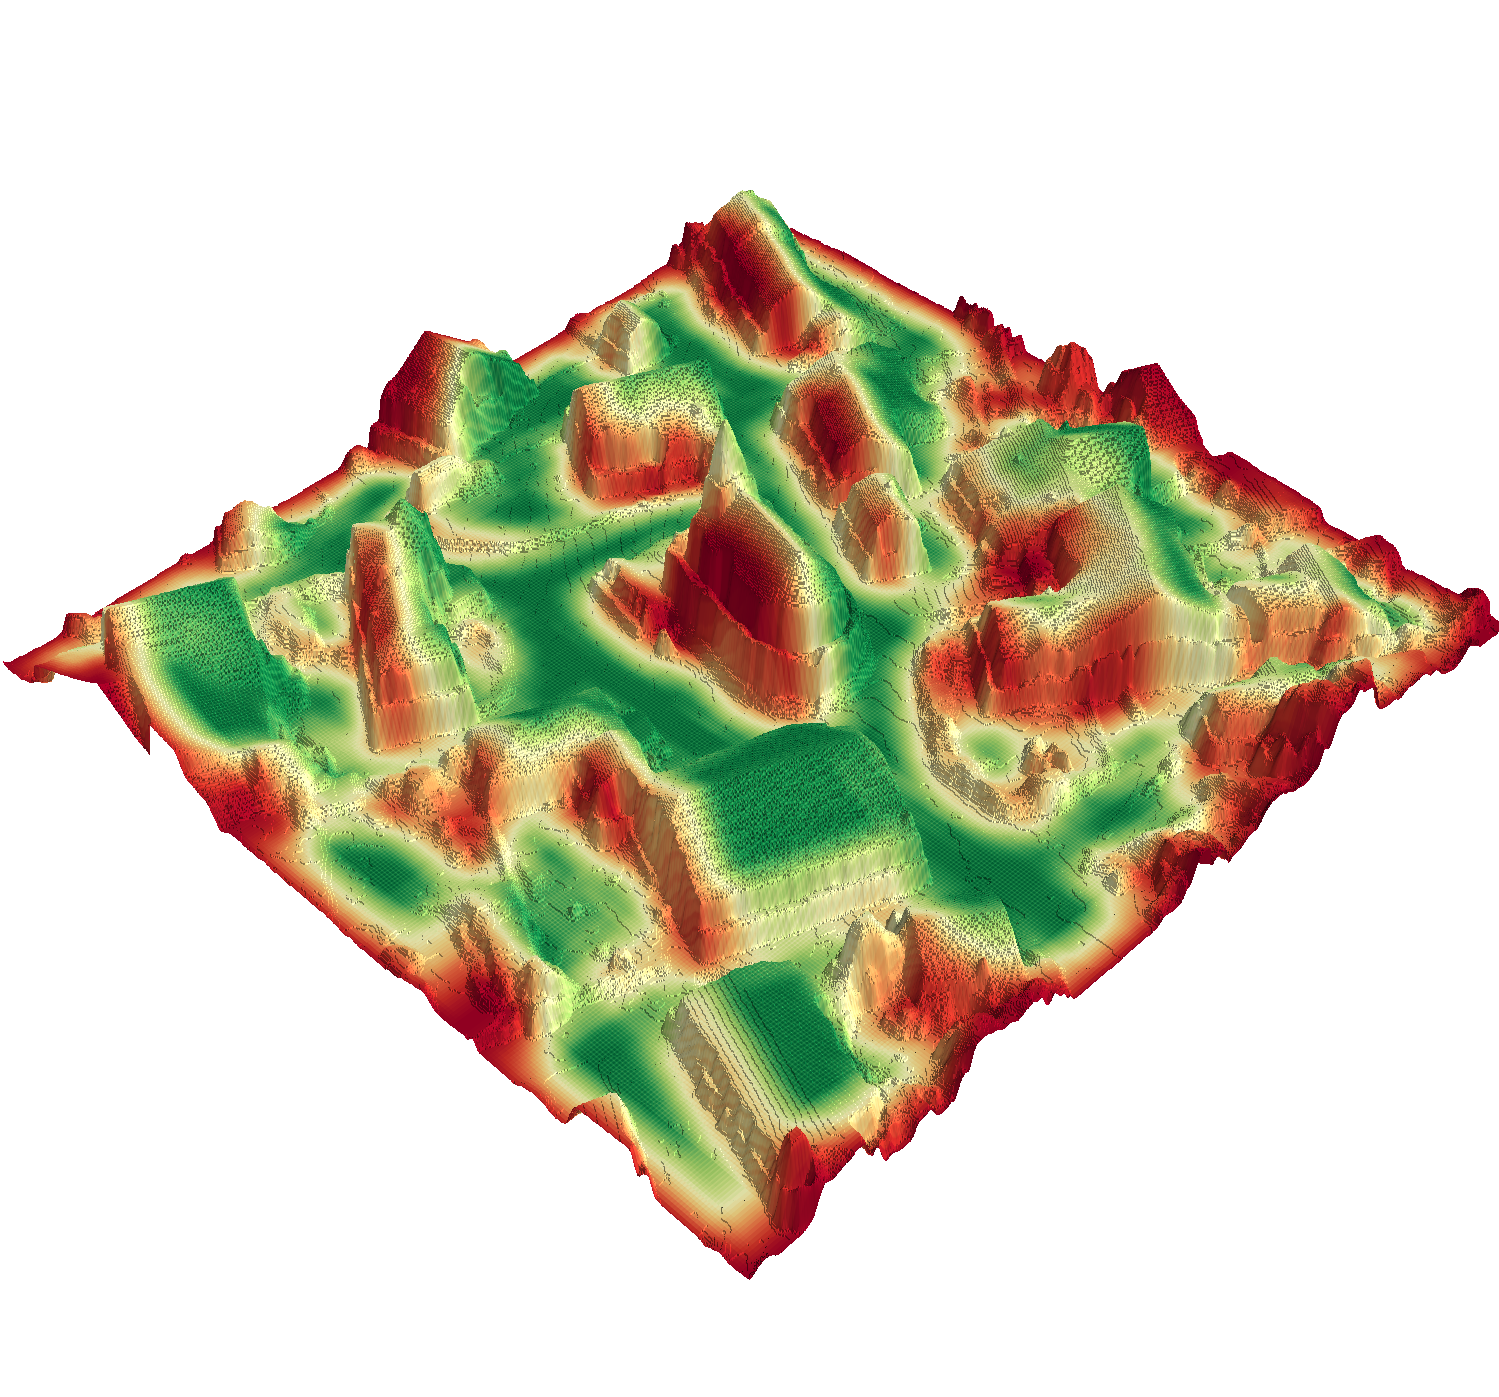
\includegraphics[width=\linewidth]{../img/4/traversability/sullens/-270.png} 
    \subcaption{Robot moving from bottom to top} 
    % \label{fig: sullens-b2t}
  \end{subfigure}
  \begin{subfigure}[b]{0.45\textwidth}
      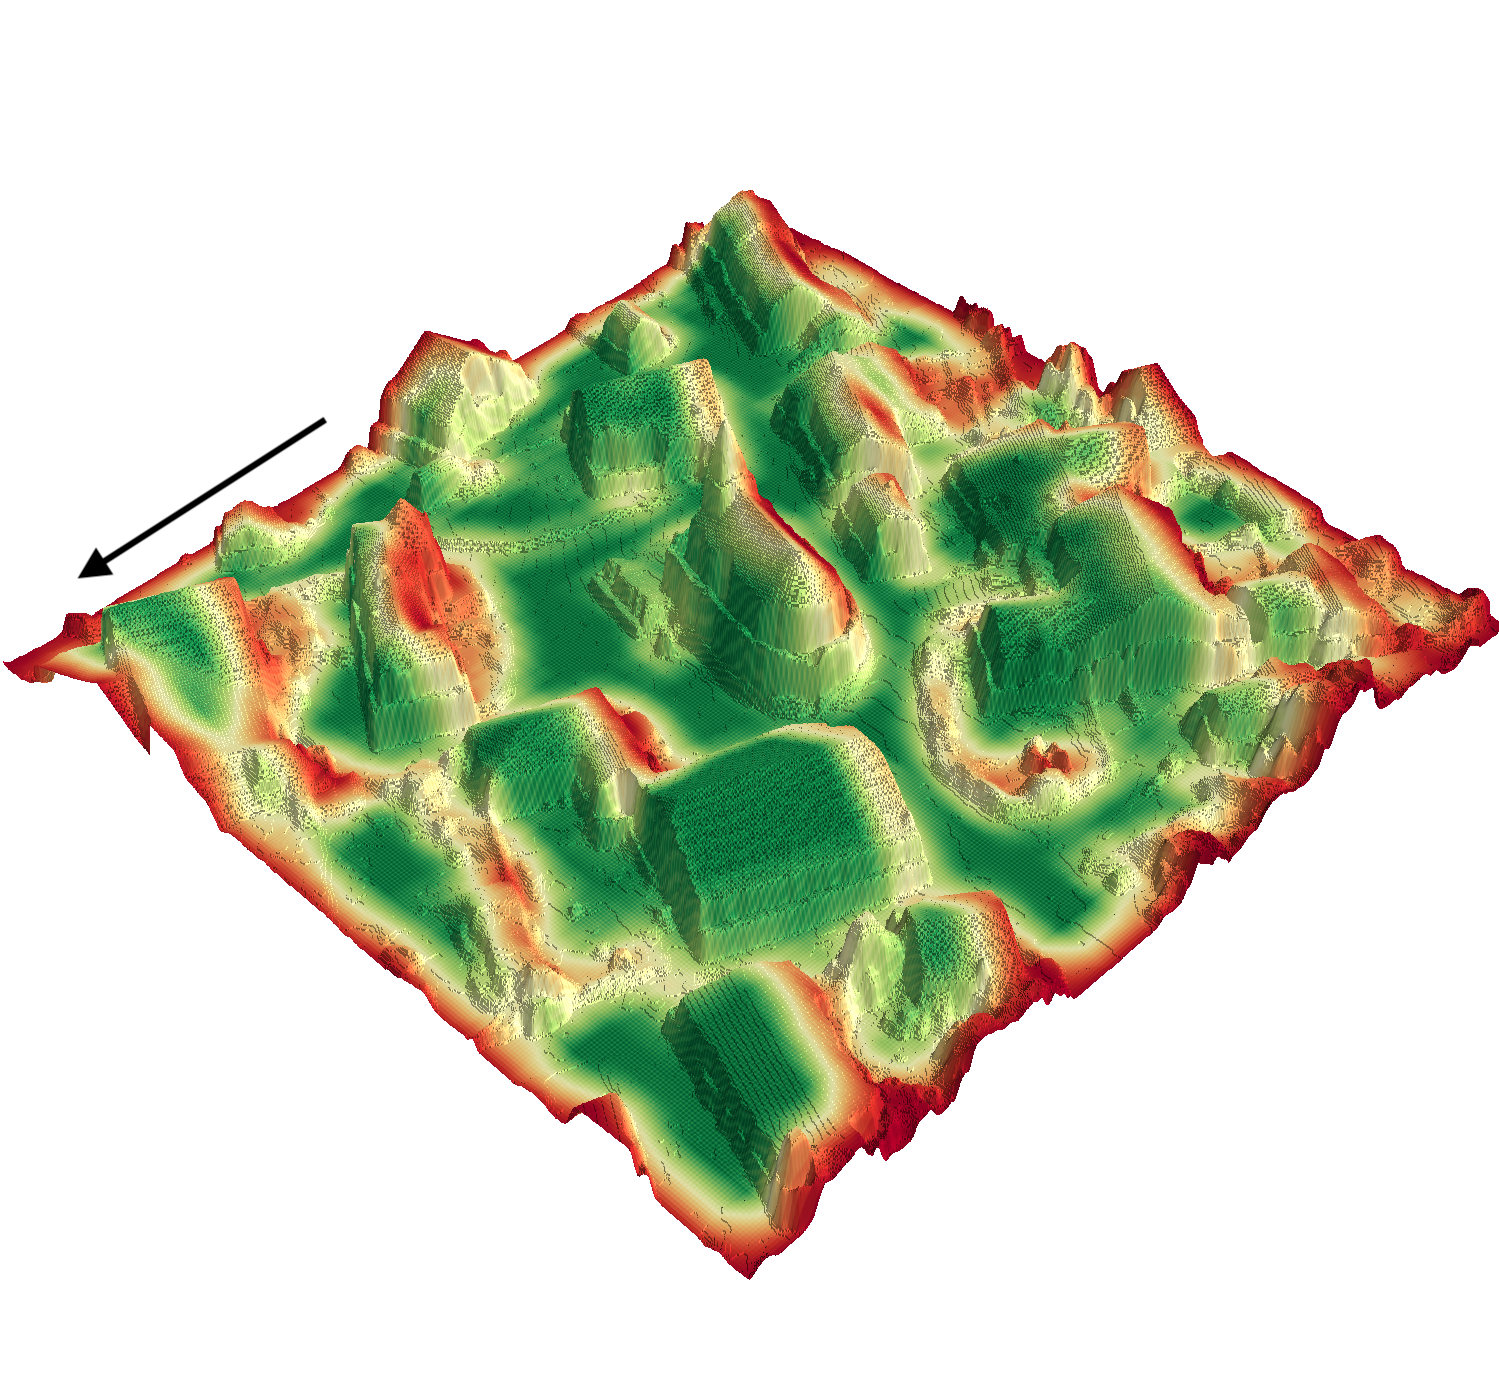
\includegraphics[width=\linewidth]{../img/4/traversability/sullens/-90.png}
      \subcaption{Robot moving from top to bottom} 
      % \label{fig: sullens-t2b}
  \end{subfigure}
  \begin{subfigure}[b]{0.45\textwidth}
    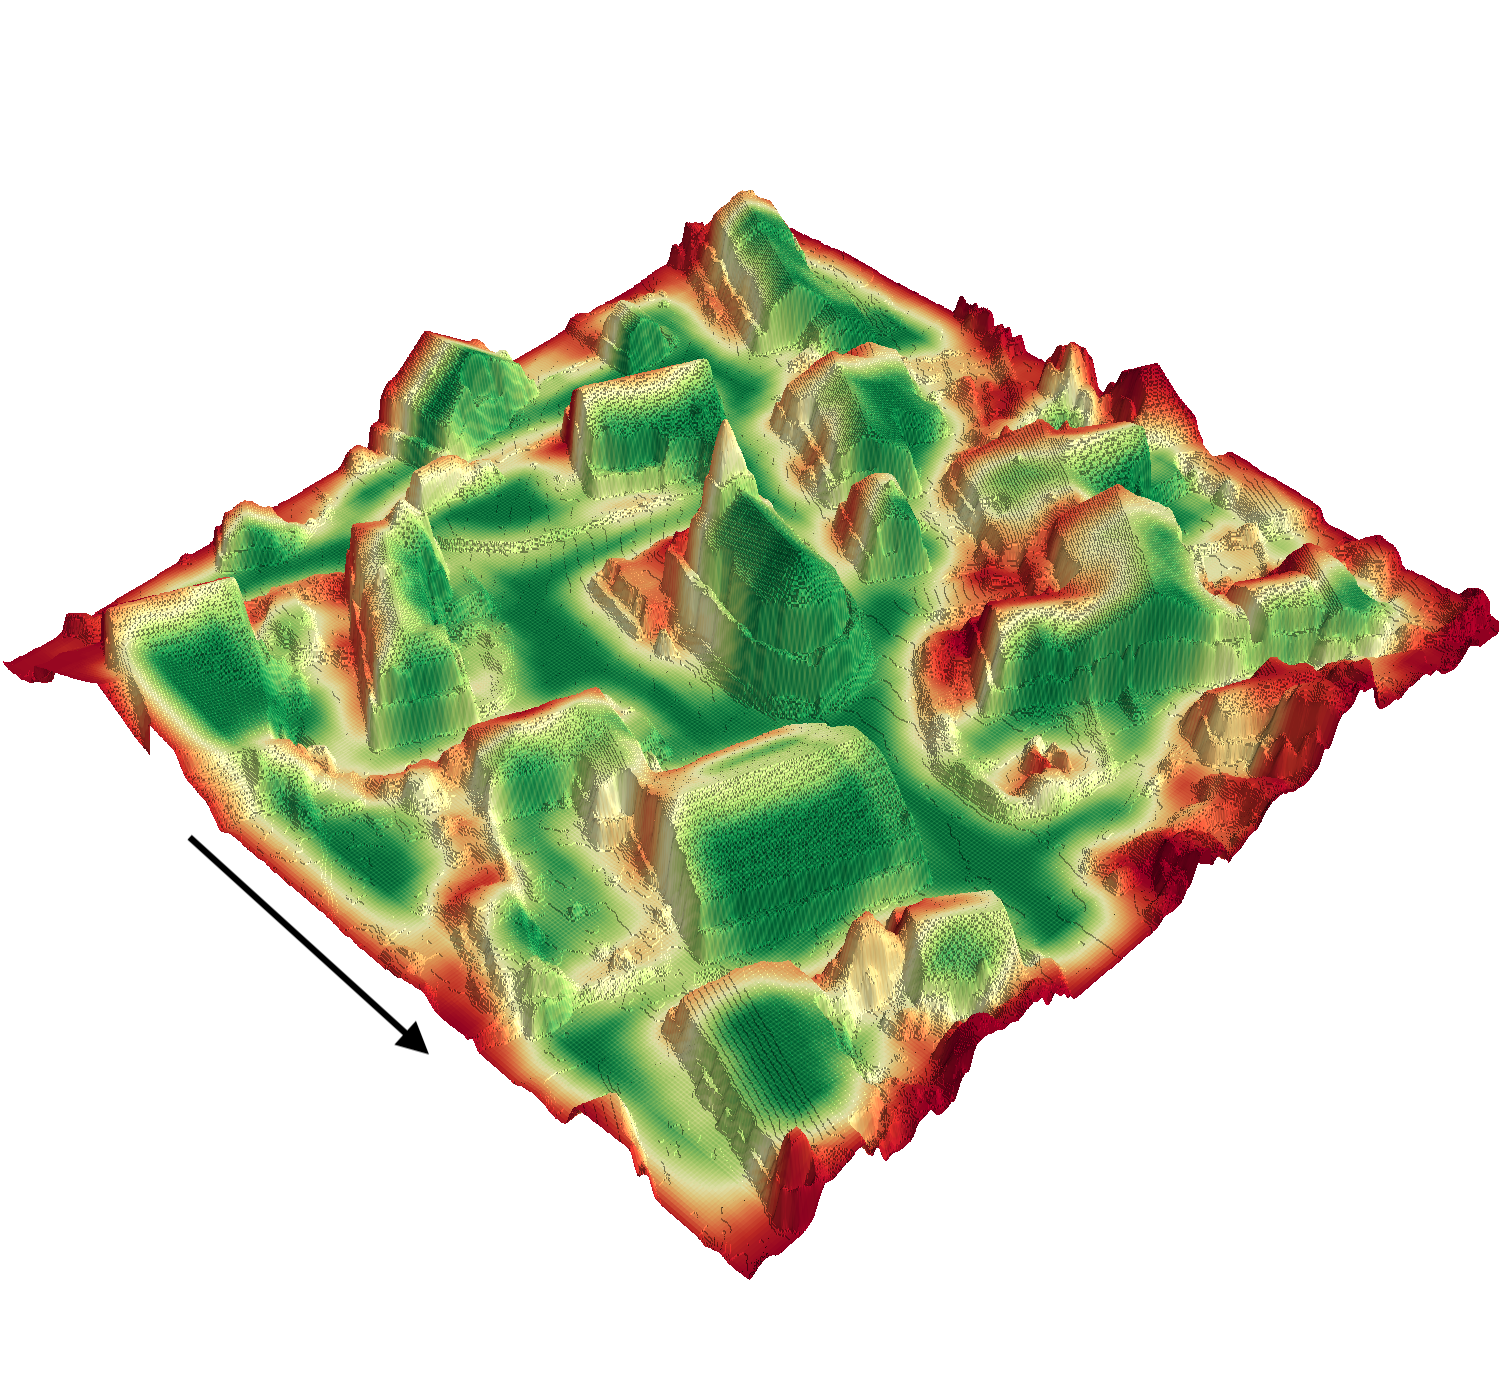
\includegraphics[width=\linewidth]{../img/4/traversability/sullens/-0.png}
    \subcaption{Robot moving from left to right}   
    % \label{fig: sullens-l2r}
  \end{subfigure}
  \begin{subfigure}[b]{0.45\textwidth}
      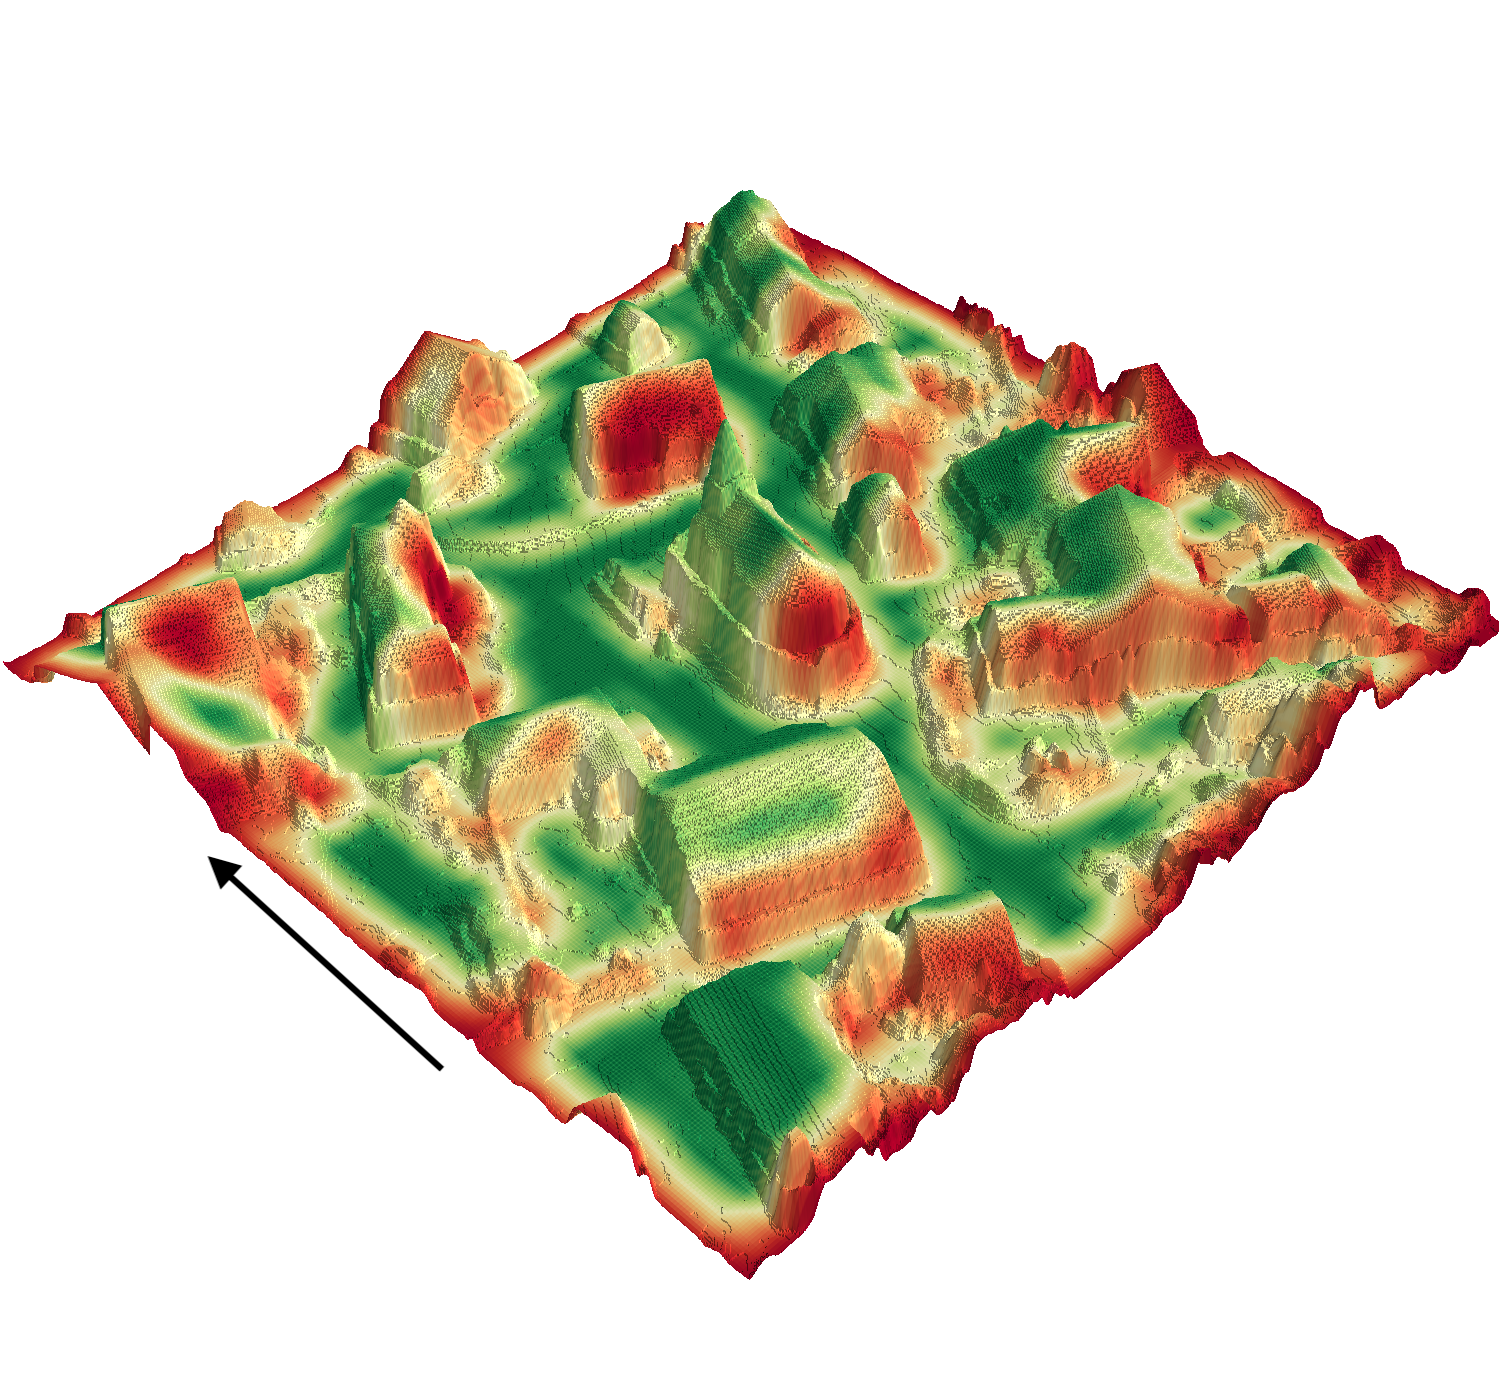
\includegraphics[width=\linewidth]{../img/4/traversability/sullens/-180.png}  
      \subcaption{Robot moving from right to left} 
      % \label{fig: bars-r2l}
  \end{subfigure}
  \caption{Traversability probability on the map of a small village for different Krock's rotation. The surface covers $30\times 30$m and has a maximum height of $10$m.}
  \label{fig : small-village-trav}
  \end{figure}
  All the streets are labeled as traversable, while some buildings' roofs (e.g. the church's one) are traversable depending on the Krock orinetation. For example, most steep roofs are not traversable when walking uphill. On the other hand, if krock walks side by side they can be traversed. Figure \ref{fig : small-village-roof-trav} shows this behavior on the church's roof.
  \begin{figure} [htbp]
    \centering
    \begin{subfigure}[b]{0.45\textwidth}
      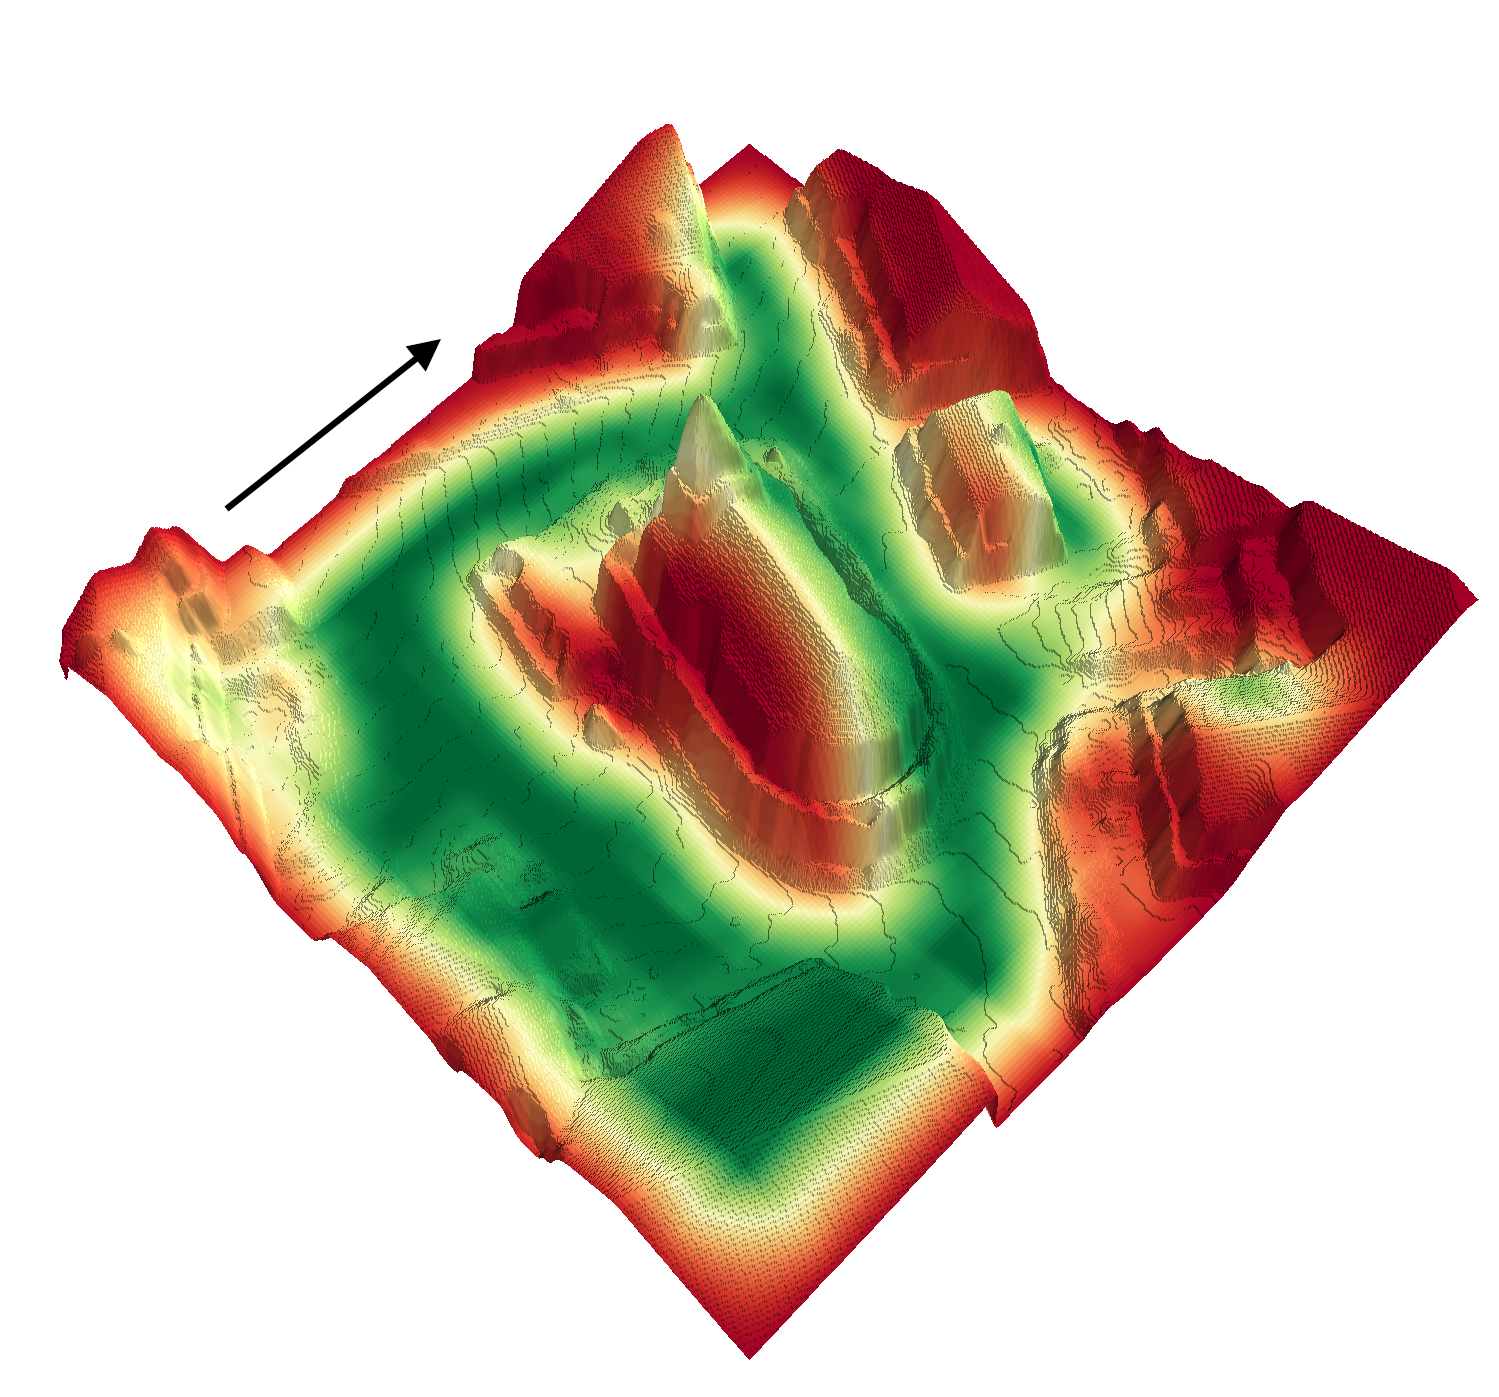
\includegraphics[width=\linewidth]{../img/4/traversability/sullens-church/-270.png} 
      \subcaption{Robot moving from bottom to top} 
      % \label{fig: sullens-b2t}
    \end{subfigure}
    \begin{subfigure}[b]{0.45\textwidth}
        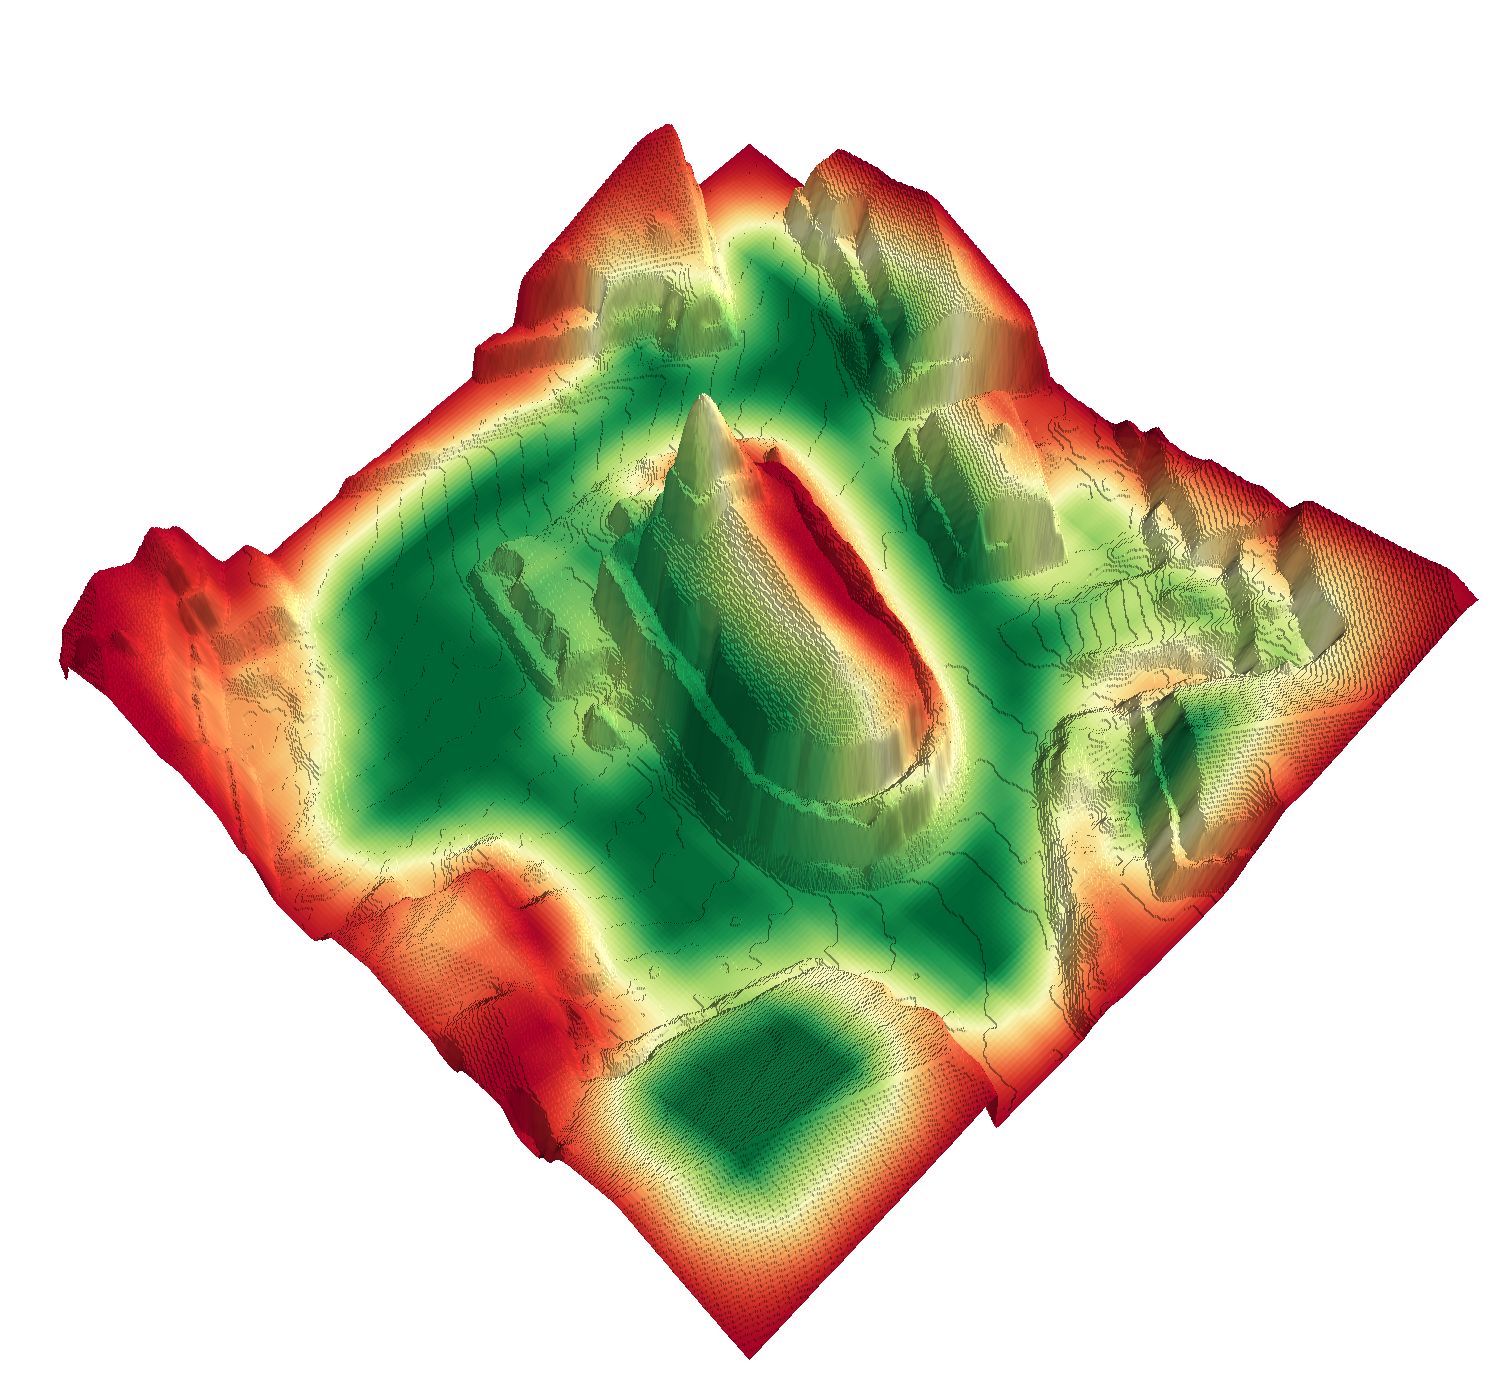
\includegraphics[width=\linewidth]{../img/4/traversability/sullens-church/-90.png}
        \subcaption{Robot moving from top to bottom} 
        % \label{fig: sullens-church-t2b}
    \end{subfigure}
    \begin{subfigure}[b]{0.45\textwidth}
      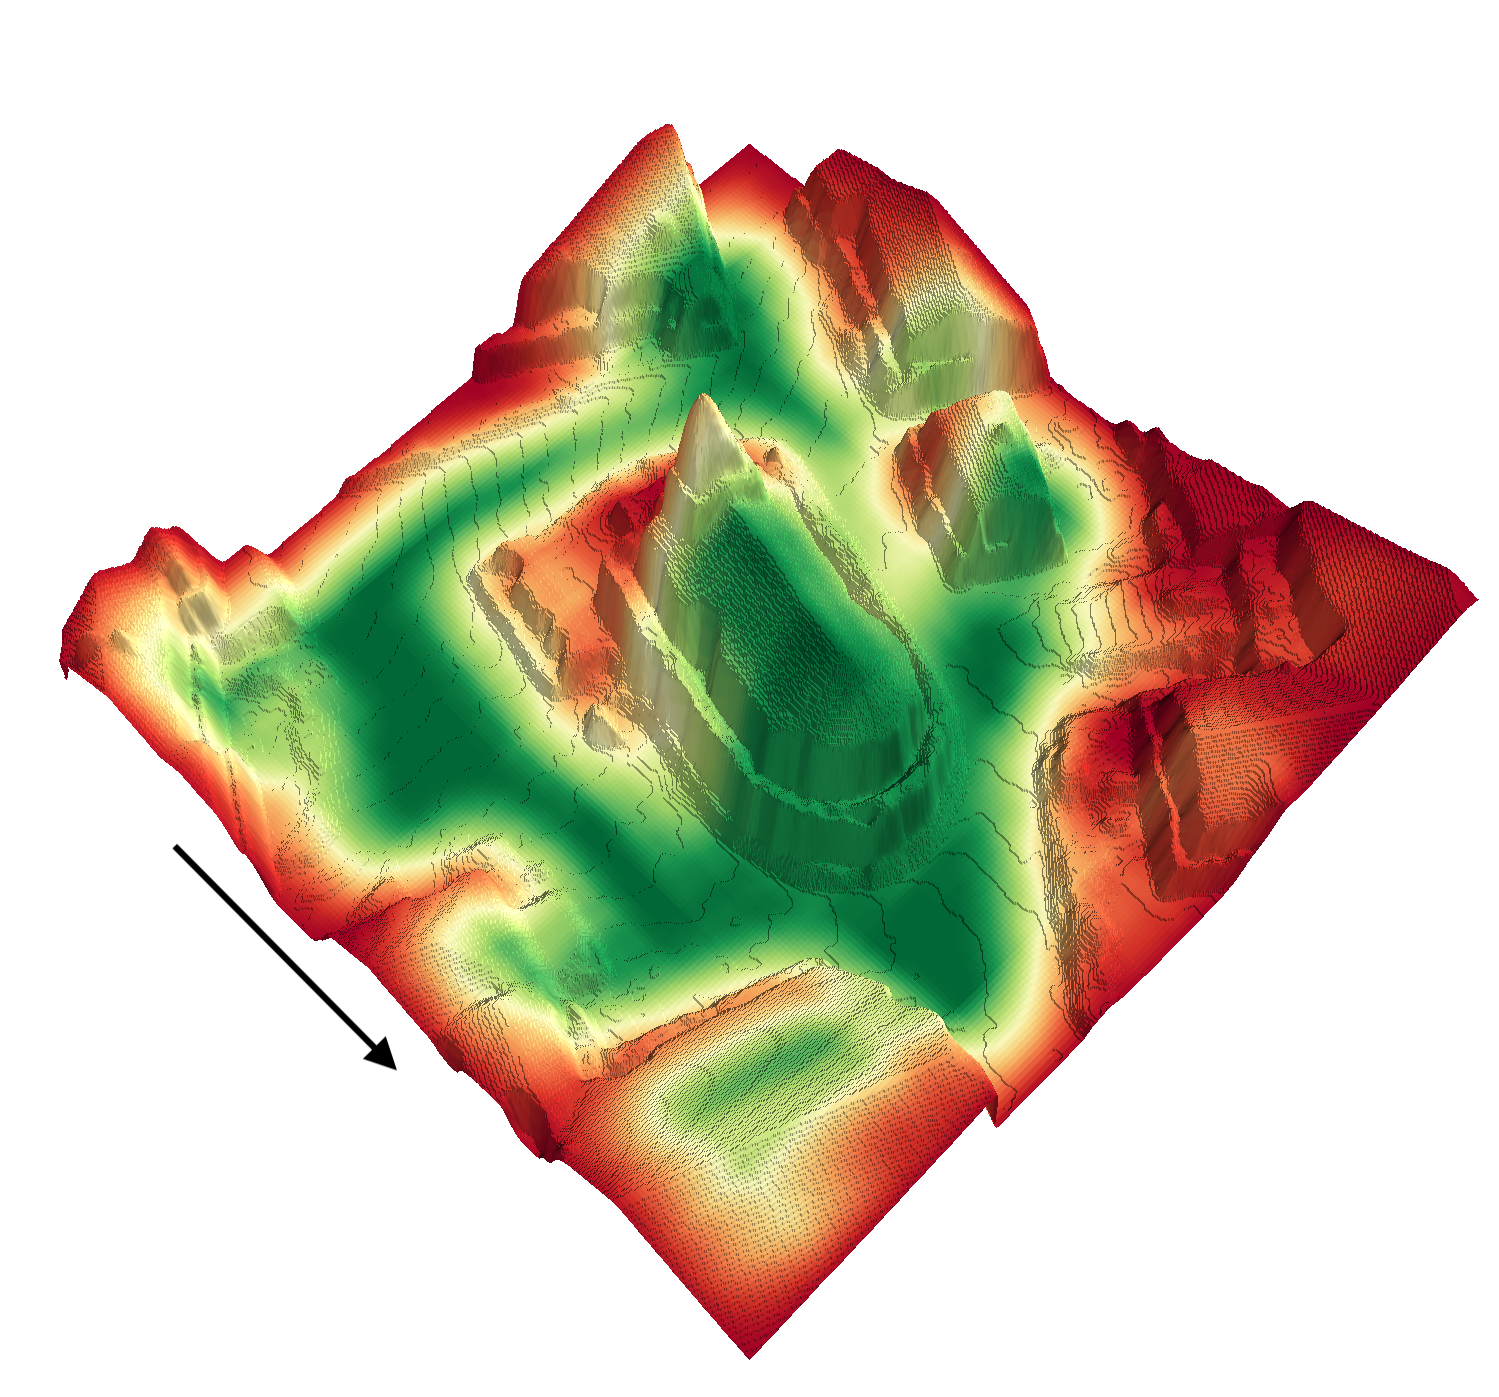
\includegraphics[width=\linewidth]{../img/4/traversability/sullens-church/-0.png}
      \subcaption{Robot moving from left to right}   
      % \label{fig: sullens-church-l2r}
    \end{subfigure}
    \begin{subfigure}[b]{0.45\textwidth}
        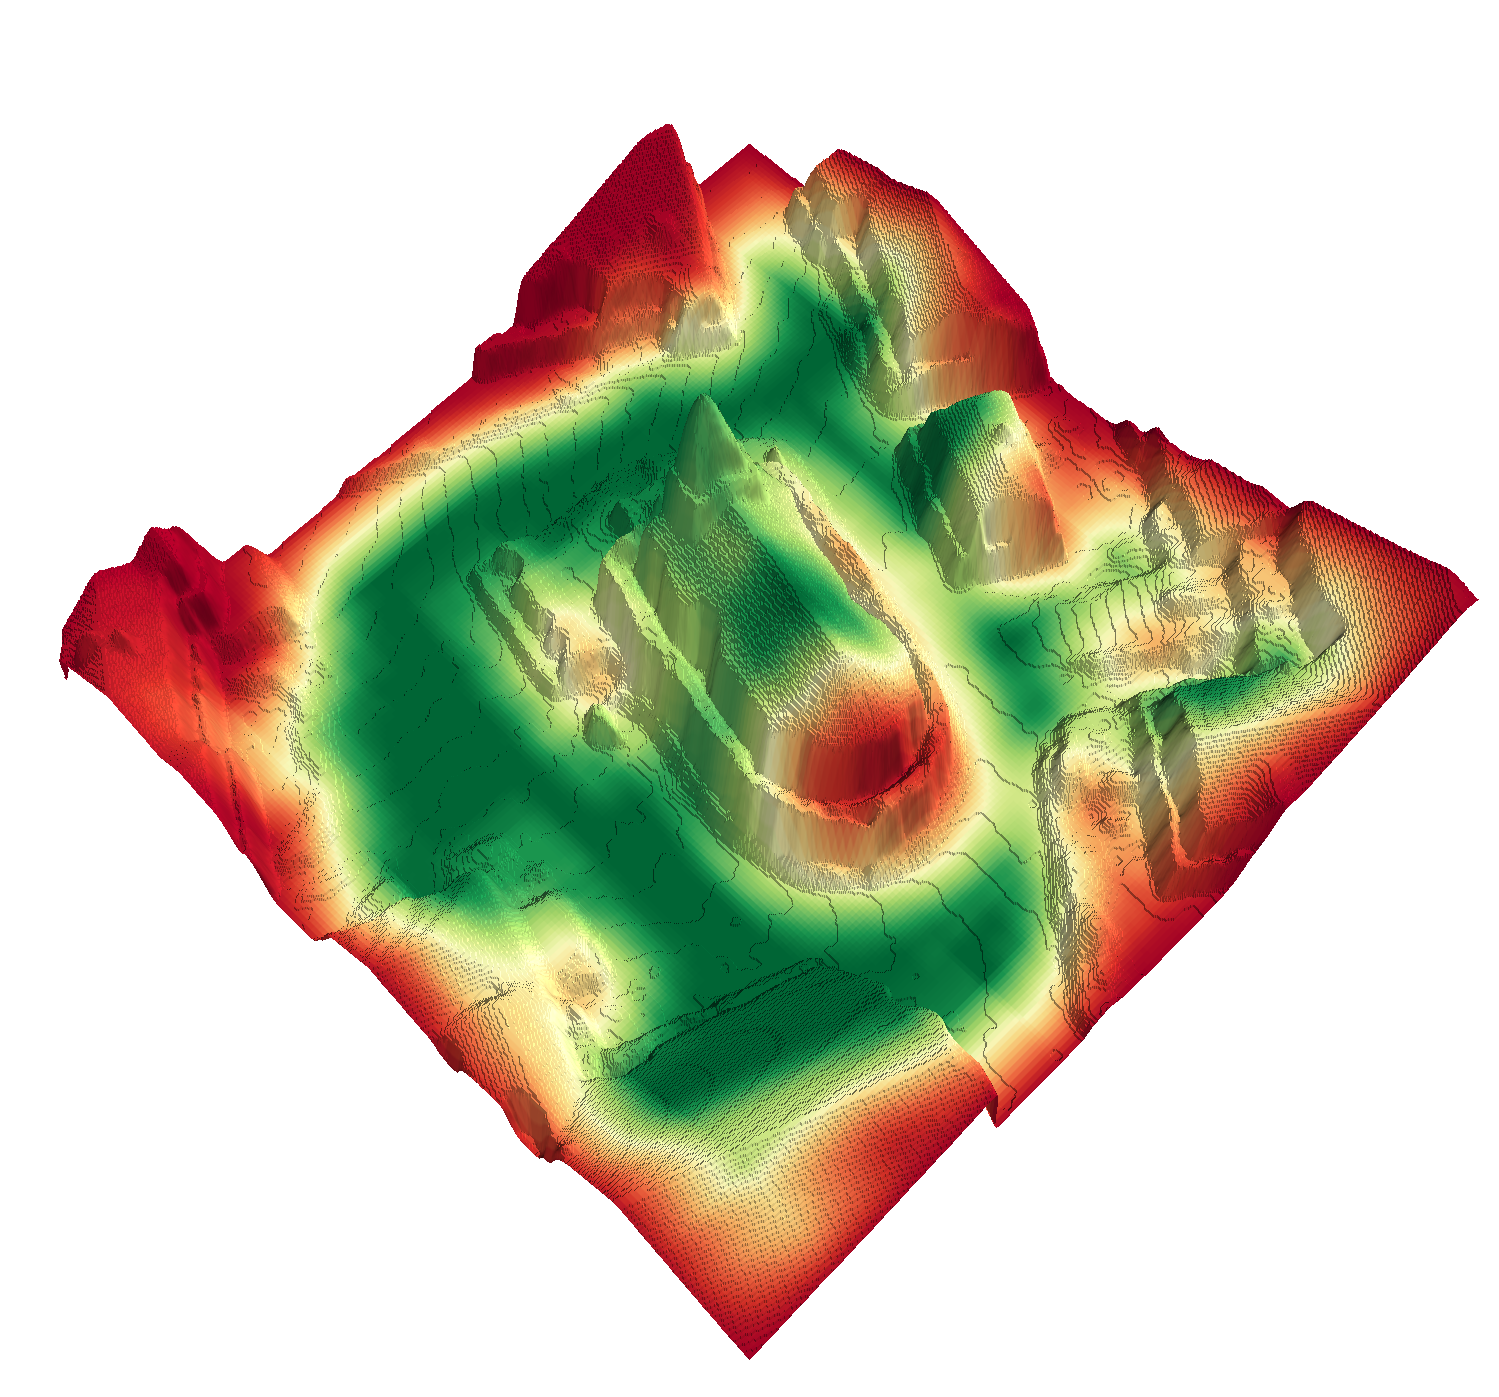
\includegraphics[width=\linewidth]{../img/4/traversability/sullens-church/-180.png}  
        \subcaption{Robot moving from right to left} 
        % \label{fig: bars-r2l}
    \end{subfigure}
    \caption{Detail of the church in the small village map for different Krock's rotation. All the fours images are correctly labeled accordingly to the robot orientation. In the first two images only downhill part of the roof is traversable. While in the last two the robot is able to travel till the end.}
    \label{fig :  small-village-roof-trav}
    \end{figure}
\end{document}